% !TeX root = ../main.tex

\chapter{研究方法}

本章為研究方法,首先對本文的研究流程進行概述,並針對流程中的數據資料蒐集、風力發電預測與收益模型分析等步驟,進一步介紹與說明所使用到的原理與方法,而模型建構與實現的細節則留待後續章節中提到時再進行詳細敘述。

\section{研究流程概述}

本文的研究流程大致上可以劃分成數據資料蒐集、風力發電預測與收益模型分析三個步驟。數據資料蒐集部分,蒐集我國再生能源發電廠址資料與對應地區鄰近的中央氣象局歷史風速,作為後續風力預測以及案例分析中模擬計算的依據;風力發電預測部分,主要目的在於推估風力電場在不同時刻的發電數量,提供收益最佳化模型進行求解;收益模型分析部分,根據預測所得的各時刻風力機組預測發電數量,進行有限移動時域下的模型預測控制規劃求解。

\section{風力發電預測}

風力發電預測部分,將過去風速資料透過時間序列建構風速預測模型,用以推估未來某一時刻 $t$ 的風速 $v(t)$,並根據風力機組模型轉換為對應的發電功率 $p_{wt}(t)$。其中使用的時間序列組合預測模型,是先透過小波轉換將時間序列進行分解,並分別將分解後的高頻與低頻訊號建立整合自迴歸移動平均模型與支持向量迴歸模型,最後再將預測結果進行重構。

\subsection{小波時頻分析}

短期風速預測的時間跨度較小,通常不考慮季節性影響,本研究中的時間序列分解將採用訊號處理中經常使用的小波轉換 (Wavelet Transform, WT) 作為處理工具,其概念與傅立葉轉換 (Fourier Transform, FT) 類似,目前被廣泛用於量子力學、醫學影像與機器診斷等領域。

\subsubsection{傅立葉轉換 (Fourier Transform, FT)}

傅立葉轉換是一種線性積分轉換,可以將訊號由時域 (time domain) 轉換為頻域 (frequency domain),假設 $x(t)$ 是滿足可積分條件的時間訊號,使用 $e^{-i \omega t}$ 的弦波訊號進行組成,則其傅立葉轉換的積分表示式如方程式 \eqref{equation: Fourier Transform} 所示。
% Equation: Fourier Transform
\begin{equation}\label{equation: Fourier Transform}
  \mathcal{FT}\{ x(t) \} = \int_{-\infty}^{\infty} x(t) e^{-i \omega t} \, \diff t
\end{equation}
%
由於捨棄了時域的資訊,因此無法從上述的傅立葉轉換中得到該訊號於不同時間點的頻率資訊,例如訊號發出時間、訊號是否延遲、訊號延遲時間等。針對傅立葉轉換無法傳達時間變化頻率的缺陷,在 \cite{mallat1989theory} 中提出了添加窗函數 (window function) 的短時傅立葉轉換 (Short-Time Fourier Transform, STFT) 以進行分析,使用 $\omega(t - \tau)$ 作為窗函數的短時傅立葉轉換積分式如方程式 \eqref{equation: Short-Time Fourier Transform} 所示。
% Short-Time Fourier Transform
\begin{equation}\label{equation: Short-Time Fourier Transform}
  \mathcal{STFT}\{ x(t, \tau) \} = \int_{-\infty}^{\infty} x(t) \omega(t - \tau) e^{-i \omega t} \, \diff t
\end{equation}
%
採用不同寬度的窗函數會在時域與頻域上有不同的解析度:較寬的窗函數有較高的頻域解析度,但時域解析度較低;較窄的窗函數有較高的時域解析度,但頻域解析度較低。小波轉換的積分表示式如方程式 \eqref{equation: Wavelet Transform} 所示,使用了一組具有震盪特性且能夠迅速衰減至零的小波母函數 (mother wavelet) 逼近目標函數,以解決短時傅立葉轉換中的窗函數由於大小與形狀固定,在應對不同頻率訊號時的侷限性。
% Equation: Wavelet Transform
\begin{equation}\label{equation: Wavelet Transform}
  \mathcal{WT}\{ x(a, b) \} = \int_{-\infty}^{\infty} x(t) \psi_{a, b}(t)
\end{equation}
%
其中,$\psi_{a,b} (t)$ 是作為轉換基底的小波母函數。如方程式 \eqref{equation: Mother Wavelet} 所示,式中尺度參數 $a$ 表示週期長度,平移參數 $b$ 表示移動長度,分別代表空間軸上的縮放與時間軸上的平移,滿足 $a, b \in \mathbb{R}$ 且 $a \neq 0$。
% Equation: Mother Wavelet
\begin{equation}\label{equation: Mother Wavelet}
  \psi_{a, b}(t) = \frac{1}{\sqrt{\abs{a}}} \psi \left( \frac{t-b}{a} \right)
\end{equation}
%
為滿足小波分解在不同領域應用下的需求差異,學者提出了眾多的小波母函數如 Daubechies 小波、Symlet 小波與 Coiflet 小波等。在選擇小波母函數時會考慮以下性質:
%
\begin{itemize}
  \item \textbf{緊支撐 (Compactly Supported)}:當尺度函數與小波函數只在有限區間內存在非零狀態,稱其具備緊支撐性,區間寬度越大的小波函數具備較好的局部分辨與去除雜訊能力。
  \item \textbf{正交性 (Orthonormal)}:若小波係數之間的相關程度越小,分解後的訊號在重構後可以獲得較為平滑的效果。
  \item \textbf{對稱性 (Symmetric)}:影響小波基底在變換前後的偏題程度,採用具備對稱性的小波函數分解訊號,有利於訊號的恢復與重建。
  \item \textbf{消失矩 (Vanishing Moments)}:若 $\displaystyle \int \psi(t) t^m \, dt = 0$ 則稱該小波函數具有 $m$ 階的消失矩,較高的消失矩具有較好的訊號壓縮與提取資訊能力。
\end{itemize}
%
常見的小波母函數型態與特性如表 \ref{table: Wavelet Mother Function} 所示。
%
\begin{table}[htp]
  \centering
  \caption[常見小波母函數特徵]{常見小波母函數特徵}
  \begin{tabular*}{0.85\textwidth}{lccccc}
    \toprule
    \textbf{小波母函數} & \textbf{緊支撐} & \textbf{支撐寬度} & \textbf{對稱性} & \textbf{正交性} & \textbf{消失矩} \\
    \midrule
    Sinc & 否 & 無限 & 是 & 是 & 否 \\
    Harr & 是 & $1$ & 是 & 是 & $1$ \\
    Meyer & 否 & 無限 & 是 & 是 & 無限 \\
    Ricker & 否 & 無限 & 是 & 否 & $1$ \\
    Morlet & 否 & 無限 & 是 & 否 & \\
    Symlet (symN) & 是 & $2N-1$ & 近似對稱 & 是 & $N$ \\
    Coiflet (cN) & 是 & $6N-1$ & 近似對稱 & 是 & $2N$ \\
    Daubechies (dbN) & 是 & $2N-1$ & 是 & 是 & $N$ \\
    \bottomrule
  \end{tabular*}
  \label{table: Wavelet Mother Function}
\end{table}
%
\subsubsection{連續小波轉換 (Continuous Wavelet Transform, CWT)}

小波轉換中,小波母函數的取值範圍主要依賴於尺度參數與平移參數,若 $a$ 和 $b$ 在實數域中為連續,則連續小波轉換可以表示如方程式 \eqref{equation: Continuous Wavelet Transform} 所示。
%
\begin{equation}\label{equation: Continuous Wavelet Transform}
  \mathcal{CWT}\{ x(a, b) \} = \frac{1}{\sqrt{\abs{a}}} \int_{-\infty}^{\infty} x(t) \bar{\psi} \left( \frac{t - b}{a} \right) \, \diff t
\end{equation}
%
其中,$\bar{\psi}$ 為 $\psi$ 的共軛複數。在實際情況中,小波轉換應存在其反轉換才有意義,因此必須滿足方程式 \eqref{equation: Admissible Condition} 所表示的小波轉換容許性條件 (Admissible Condition),式中的 $C_{\psi}$ 稱為容許性常數 (Admissible Constant),表示如方程式 \eqref{equation: Admissible Constant} 所示。
%
\begin{equation}\label{equation: Admissible Condition}
  0 < C_{\psi} < \infty
\end{equation}
%
\begin{equation}\label{equation: Admissible Constant}
  C_{\psi} = \int_{-\infty}^{\infty} \frac{\abs{\hat{\psi} (\omega)}^2}{|\omega|} \diff \omega
\end{equation}
%
\subsubsection{離散小波轉換 (Discrete Wavelet Transform, DWT)}

離散小波轉換是為了降低連續小波轉換在計算上的複雜度而提出,經常被用於數值分析與時頻分析中,藉由將連續小波轉換公式中的尺度參數 $a$ 與平移參數 $b$ 離散化所得,即將 $a$ 和 $b$ 分別調整為 $a = a_{0}^{m}$ 與 $b = na$,則離散小波轉換可以表示如方程式 \eqref{equation: Discrete Wavelet Transform} 所示。
%
\begin{equation}\label{equation: Discrete Wavelet Transform}
  \mathcal{DWT}\{ x(m, n) \} = \frac{1}{\sqrt{\abs{a_{0}^m}}} \sum_{k=-\infty}^{\infty} x(t) \bar{\psi} \left( \frac{k - n}{a_{0}^m} \right)
\end{equation}
%
其中 $k$ 為運算指標,且 $m, n \in \mathbb{Z}, a_{0} \neq 1$,一般通常會選擇 $a_0 = 2$ 的二元化小波函數 (Dyadic Wavelet) ,此時只要選擇適當的 $m$ 值即可將訊號作細節 (detailed) 與近似 (approximate) 的分析,值得一提的是式中離散的部分僅有參數 $a$ 和 $b$,訊號本身仍為連續訊號。

藉由離散小波轉換,可以將輸入訊號分解成輸入訊號的低頻部分與高頻部分,通常以濾波器模組實現,輸入訊號先通過高通濾波器與低通濾波器後,再經由二分之一的取樣,可分別得到高頻小波係數與低頻小波係數。離散小波訊號的輸出關係通常以圖 \ref{figure: Descrete Wavelet Transform} 所示的階層式架構表示。
%
\begin{figure}[htbp]
  \centering
  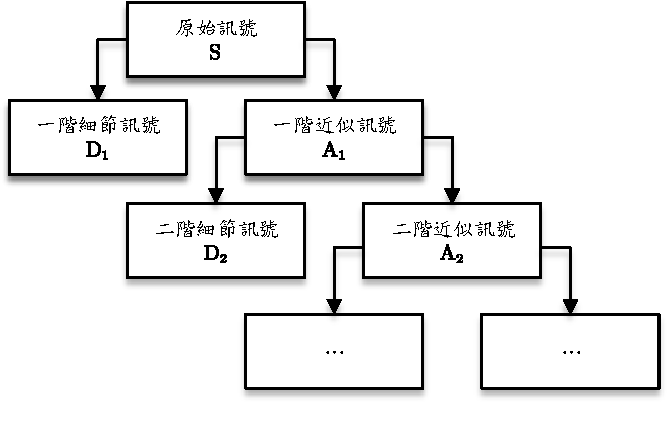
\includegraphics{descrete_wavelet_transform}
  \caption{離散小波轉換階層架構}
  \label{figure: Descrete Wavelet Transform}
\end{figure}
%
\subsection{時間序列模型}

\subsubsection{時間序列預測 (Time Series Prediction Model)}

將資料按照一定的時間間隔與發生順序紀錄而成的數列稱為時間序列 (time series) ,時間序列預測透過序列本身所具有的時序性與自相關性,基於已知事件建構數學模型找出趨勢以確定未來事件 \cite{Wang2012}。一個基本的時間序列預測模型方程式 \eqref{equation: Time Series Prediction Model} 所示 \cite{box2015time}:
% Equation: Time Series Prediction Model
\begin{equation}\label{equation: Time Series Prediction Model}
  \hat{y} (t + T) = f\Big( y(t), y(t - T), \dots, y(t - mT) \Big)
\end{equation}
%
其中,$T$ 為取樣的時間間隔;$\hat{y}(t + T)$ 為預測值;$y(t)$、$y(t - T)$、$\dots$、$y(t - mT)$ 為當下的實際觀測值與過去時刻的實際觀測值;$m$ 值決定採用之前多少時刻的觀測值來進行預測。

方程式 \eqref{equation: Time Series Prediction Model} 表示:未來某一時刻的預測值僅依賴於前 $m$ 個時刻的歷史觀測值。

\subsubsection{平穩性與非平穩性 (Stationary and Non-Stationary)}

時間序列通常存在非平穩性 (nonstationarity) 與時間波動 (time-varying volatility) 的特徵導致分析困難,若時間序列的統計特徵指標與時間無關,不會因為時間改變而變動,稱其具備平穩性或稱為恆定性。穩定性依據其形態分為強穩定性與弱穩定性,一般統計學中定義採用弱穩定性 (weakly stationary) :若時間序列 $\{ Y_t \}$ 滿足方程式 \eqref{equation: Stationary Condition},則稱時間序列 $\{ Y_t \}$ 是平穩的。
% Equation: Stationary Condition
\begin{subequations}\label{equation: Stationary Condition}
  \begin{alignat}{2}
    E(Y_t) = E(Y_{t - s}) = \mu                                                  \qquad & \text{, } \forall~t, s \in \mathbb{N}    \\
    E(Y_t - \mu)(Y_t - \mu) = E(Y_{t-s} - \mu)(Y_{t-s} - \mu) = \sigma_{y}^{2}   \qquad & \text{, } \forall~t, s \in \mathbb{N}    \\
    E(Y_t - \mu)(Y_{t-s} - \mu) = E(Y_{t-j} - \mu)(Y_{t-j-s} - \mu) = \gamma_{s} \qquad & \text{, } \forall~t, s, j \in \mathbb{N}
  \end{alignat}
\end{subequations}
%
方程式 \eqref{equation: Stationary Condition} 表示平穩時間序列的期望值 $\mu$、變異數 $\sigma_{y}^{2}$ 與自相關係數 $\gamma_r$ 均為常數,不因時間的變動而改變。

\subsubsection{模型分類}

一般而言,會將時間序列根據其是否滿足平穩性條件,分為平穩性時間序列 (Stationary Time Series) 與非平穩時間序列 (Non-stationary Time Series) ,並依此決定預測時所採用的時間序列預測模型。平穩性時間序列多採用自迴歸模型 (AR) 、移動平均模型 (MA) 或自迴歸移動平均模型 (ARMA) ;而非平穩時間序列需要透過差分運算使時間序列滿足平穩性,採用差分移動自迴歸模型 (ARIMA) ,這些模型的介紹如下:

\paragraph{自迴歸模型 (Autoregressive Model, AR Model)}

使用時間序列自身作為迴歸變數,依賴於本身延遲的滯後項與當前時間的干擾項對未來數值進行預測,其模型如方程式 \eqref{equation: AR Model} 所示,適用於平穩性時間序列。
%
\begin{equation}\label{equation: AR Model}
  \begin{split}
    \hat{y}_{t} & = c + \sum_{i = 1}^{p} \phi_{i} y_{t-i} + \epsilon_{t} \\
    & = c + \phi_{1} y_{t-1} + \phi_{2} y_{t-2} + \cdots + \phi_{p} y_{t-p} + \epsilon_{t}
  \end{split}
\end{equation}
%
其中,$c$ 為常數項;$\phi_i~(i = 1, 2, \ldots, p)$ 為自相關係數;$y_{t - i}~(i = 1, 2, \ldots, p)$ 為時間序列中過去時刻的觀測值;$\epsilon_t$ 為當前時間的干擾項,代表無法由過去時刻資料所解釋的雜訊或白噪聲;$p$ 為模型的自迴歸階數。一個 $p$ 階的自迴歸模型記為 $\text{AR} (p)$。

\paragraph{移動平均模型 (Moving-Average Model, MA Model)}

主要依賴於過去與當前時間的干擾項,對不同時期的雜訊或噪聲給予不同的權重來進行線性組合,其模型如方程式 \eqref{equation: AR Model} 所示,適用於平穩性時間序列。
%
\begin{equation}\label{equation: MA Model}
  \begin{split}
    \hat{y}_{t} & = c + \sum_{j = 1}^{q} \theta_{j} \epsilon_{t-j} + \epsilon_{t} \\
    & = c + \theta_{1} \epsilon_{t-1} + \theta_{2} \epsilon_{t-2} + \cdots + \theta_{q} \epsilon_{t-q} + \epsilon_{t}
  \end{split}
\end{equation}
%
其中,$\mu$ 為時間序列的平均值;$\theta_{j}~(j = 1, 2, \ldots, q)$ 為移動平均係數;$\epsilon_{t - j}~(j = 1, 2, \ldots, q)$ 和 $\epsilon_t$ 分別為時間序列中過去時刻與當前時間的干擾項,代表雜訊或白噪聲;$q$ 為模型的滑動平均階數。一個 $q$ 階的移動平均模型記為 $\text{MA} (q)$。

\paragraph{自迴歸移動平均模型 (Autoregressive Moving-Average Model, ARMA Model)}

採用了自迴歸模型與移動平均模型作為基礎,可以視為是兩個模型的線性組合,其模型如方程式 \eqref{equation: ARMA Model} 所示,適用於平穩性時間序列。
%
\begin{equation}\label{equation: ARMA Model}
  \hat{y}_{t} = \mu + \sum_{i = 1}^{p} \phi_{i} y_{t-i} + \sum_{j = 1}^{q} \theta_{j} \epsilon_{t-j} + \epsilon_{t}
\end{equation}
%
其中,分別引入了方程式 \eqref{equation: AR Model} 與 \eqref{equation: MA Model} 所表示自迴歸模型與移動平均模型。一個包含了 $p$ 階自迴歸項和 $q$ 階的移動平均項的自迴歸移動平均模型記為 $\text{ARMA} (p, q)$。

\paragraph{整合自迴歸移動平均模型 (Autoregressive Integrated Moving-Average Model, ARIMA Model)}

將非平穩時間序列透過方程式 \eqref{equation: First Order Difference Series} 的差分處理,使其具備平穩性之後再建立自迴歸移動平均模型,其模型如方程式 \eqref{equation: ARIMA Model} 所示,適用於非平穩性時間序列。
%
\begin{gather}
  \label{equation: First Order Difference Series}
  {y}_{t}^{(d)} = y_{t}^{(d-1)} - y_{t-1}^{(d-1)} \\[1em]
  \label{equation: ARIMA Model}
  \hat{y}_{t}^{(d)} = c + \sum_{i = 1}^{p} \phi_{i} {y}_{t-i}^{(d)} + \sum_{j = 1}^{q} \theta_{j} \epsilon_{t-j} + \epsilon_{t}
\end{gather}
%
其中,分別引入了方程式 \eqref{equation: AR Model} 和 \eqref{equation: MA Model} 所表示自迴歸模型與移動平均模型,並使用差分處理後的時間序列進行預測;$d$ 表示整合階數。一個經 $d$ 次差分後方使具備平穩性,包含了 $p$ 階自迴歸項和 $q$ 階的移動平均項的整合自迴歸移動平均模型記為 $\text{ARIMA} (p, d, q)$。

\subsubsection{平穩性檢驗 (Stationary Testing)}

實務上在檢驗時間序列的平穩性時,會使用圖形檢驗法或單根檢驗法。圖形檢驗法透過觀察時間序列的走勢圖來判斷是否存在趨勢性與週期性,根據觀察者不同而有主觀性差異;單根檢驗法透過比較時間序列特徵根與單位圓位置關係判斷平穩性,實證分析中常用的單根檢定方法有:Dickey-Fuller 檢定 (DF 檢定) 、Augmented Dickey-Fuller 檢定 (ADF 檢定) 、Phillips-Perron 檢定 (PP 檢定) 、Kwiatkowski, Phillips, Schmidt \& Shin 檢定 (KPSS 檢定) 、Elliott-Rothenberg-Stock Point-Optimal 檢定 (ERS Point-Optimal 檢定) 和 Ng-Perron 檢定 (NP 檢定) 等,以下針對本研究中所使用的 ADF 檢定與 KPSS 檢定進行說明。

\paragraph{Augmented Dickey-Fuller 檢定 (ADF 檢定)}

延伸自 DF 檢定,修正了一般 DF 檢定只能用於檢驗一階時間序列相關穩定性的設定,因此可以用於檢測存在高階時間序列相關的穩定性。根據常數項或時間趨勢的有無,分為以下三種型態:
%
\begin{itemize}
  \item \textbf{無常數項以及時間趨勢} \\
        \begin{equation}
          \hat{y}_{t} = \beta y_{t - 1} + \sum_{j = 1}^{p - 1} \zeta_{j} \Delta y_{t - j} + \epsilon_{t} \quad \text{, } \epsilon_{t} \sim \mathcal{WN}(0, \sigma^2)
        \end{equation}
  \item \textbf{含常數項但無時間趨勢} \\
        \begin{equation}
          \hat{y}_{t} = \mu + \beta y_{t - 1} \sum_{j = 1}^{p - 1} \zeta_{j} \Delta y_{t - j} + \epsilon_{t} \quad \text{, } \epsilon_{t} \sim WN(0, \sigma^2)
        \end{equation}
  \item \textbf{含常數項以及時間趨勢} \\
        \begin{equation}
          \hat{y}_{t} = \mu + \alpha t + \beta y_{t - 1} + \sum_{j = 1}^{p - 1} \zeta_{j} \Delta y_{t - j} + \epsilon_{t} \quad \text{, } \epsilon_{t} \sim WN(0, \sigma^2)
        \end{equation}
\end{itemize}
%
對於上述三個迴歸模型,其假設檢定為虛無假設 $H_0$:$\beta = 1$,對立假設 $H_1: \beta < 1$,若取 $y_{t-1}$ 項 OLS 估計法下的 $t$ 檢驗值作為 ADF 統計量值,如果 ADF 統計量小於臨界值,則說明其足夠小可以拒絕虛無假設,表示時間序列具備平穩性。

\paragraph{Kwiatkowski, Phillips, Schmidt \& Shin 檢定 (KPSS 檢定)}

有別於其他單根檢定法將虛無假設設為序列具有單根而傾向接受單根,改以變數滿足平穩作為其虛無假設,通常用來確認其他單根檢定法的檢定結果。假設迴歸模型如方程式 \eqref{equation: KPSS Regression} 所示:
%
\begin{equation}\label{equation: KPSS Regression}
  \hat{y}_{t} = \zeta t + u_{t}  + \epsilon_{t}
\end{equation}
%
其中 $\zeta_t$ 為一定向趨勢;$u_{t}$ 為一隨機漫步,即 $u_{t} = u_{t-1} + u_{t}$ 且 $u_t$ 為滿足獨立有共同分佈 (independent and identically distributed)  $i.i.d. (0, \sigma_{u}^{2})$ 的隨機變數;$\epsilon_{t}$ 為一定態白噪音。假設檢定為虛無假設 $H_0$:$\sigma_{u}^{2} = 0$,對立假設 $H_1: \sigma_{u}^{2} > 1$,在此虛無假設為真的前提下可以推導出方程式 \eqref{equation: KPSS LM} 所示的 KPSS 檢定統計式。
%
\begin{equation}\label{equation: KPSS LM}
  LM = \frac{\sum_{t = 1}^{T} S_{t}^{2}}{\hat{\sigma}_{\epsilon}^{2}}
\end{equation}
%
其中 $S_t$ 為殘差的累計總合;$\hat{\sigma}_{\epsilon}^{2}$ 為長期殘差變異數的估計值,在 KPSS 檢定中採用 Bartlett windows 準則來構建加權函數 $w(s, l) = 1 - s/(l + 1)$。KPSS 檢定法推導出上述檢定統計量的漸進分配並模擬出臨界值表,此檢定為右尾檢定,若檢定落於臨界值外則拒絕虛無假設,表示時間序列不具備平穩性,需進行差分處理。

\subsubsection{模型識別 (Model Identification)}

前述所介紹的各個時間序列預測模型,最終皆能夠以整合自迴歸移動平均模型表示為 $\text{ARIMA}(p, d, q)$ 的形式,表 \ref{table: Special Case of ARIMA(p, q, r)} 為整合自迴歸移動平均模型在選用特定階數時的特例與退化後的結果。

\begin{table}[htbp]
  \centering
  \caption[整合自迴歸移動平均模型的特例]{整合自迴歸移動平均模型的特例}
  \begin{tabular*}{\textwidth}{cl}
    \toprule
    \textbf{特例}           & \textbf{說明} \\
    \midrule
    $\text{ARIMA}(0, 0, 0)$ & 白噪聲 (white noise)  \\
    $\text{ARIMA}(0, 1, 0)$ & 隨機漫步模型 (random walk)  \\
    $\text{ARIMA}(p, 0, 0)$ & 自迴歸模型 (AR Model)  \\
    $\text{ARIMA}(0, 0, q)$ & 移動平均模型 (MA Model)  \\
    $\text{ARIMA}(p, 0, q)$ & 自迴歸移動平均模型 (ARMA Model)  \\
    \bottomrule
  \end{tabular*}
  \label{table: Special Case of ARIMA(p, q, r)}
\end{table}

所謂的模型識別 (model identification) ,即是指決定整合自迴歸移動平均模型 $\text{ARIMA}(p, d, q)$ 中階數 $p, d$ 和 $q$ 的過程,此一階段將採用 Box-Jenkins 方法,透過自相關函數 (Autocorrelation Function, ACF) 與偏自相關函數 (Partial Autocorrelation Function, PACF) 及其對應的相關圖形進行判斷。

\paragraph{自相關函數 (Autocorrelation Function, ACF)}

反映了同一時間序列在不同時刻取值的相關程度,定義為第 $k$ 個時間差的自協方差函數與標準差的商值,如方程式 \eqref{equation: Autocorrelation Function} 所示。
%
\begin{equation}\label{equation: Autocorrelation Function}
  \rho_{k} = \frac{\mathrm{Cov}(y_t, y_{t + k})}{\sqrt{\mathrm{Var}(y_{t})\mathrm{Var}(y_{t+k})}} = \frac{\gamma_{k}}{\sigma_{y}^{2}}
\end{equation}
%
對於 $\text{AR}(p)$ 模型而言,其自相關函數會隨著階數 $p$ 的增加而逐步衰減但不為零,呈現拖尾 (tail off) 的性質;而對於 $\text{MA}(q)$ 模型而言,其自相關函數會在階數 $q$ 之後為零,呈現截尾 (cut off) 的性質。

\paragraph{偏自相關函數 (Partial Autocorrelation Function, PACF}

定義為移除額外變數的影響後,時間序列 $\{ y_t \}$ 與滯後 $k$ 階時間序列 $\{ y_{t-k} \}$ 的線性相關程度,通常以 $\phi_{kk}$ 來表示時間序列的偏自相關函數,定義如方程式 \eqref{equation: Partial Autocorrelation Function} 所示。
%
\begin{equation}\label{equation: Partial Autocorrelation Function}
  \phi_{kk} = \frac{\mathrm{Cov}(y_t, y_{t-k} | y_{t-1}, y_{t-2}, \cdots, y_{t-k+1})}{\sigma_{y_{t} | y_{t-1}, y_{t-2}, \cdots, y_{t-k+1}} \sigma_{y_{t-k} | y_{t-1}, y_{t-2}, \cdots, y_{t-k+1}}}
\end{equation}
%
對於 $\text{AR}(p)$ 模型而言,其偏自相關函數會在階數 $q$ 之後為零,呈現截尾 (cut off) 的性質;而對於 $\text{MA}(q)$ 模型而言,其偏自相關函數會隨著階數 $p$ 的增加而逐步衰減但不為零,呈現拖尾 (tail off) 的性質。

由於平穩時間序列的自相關函數與偏自相關函數分別具有不同特徵,在進行模型識別的過程中通常觀察其自相關函數圖形與偏自相關函數圖形的特徵,比如是否截尾以及在何處截尾來決定模型的類型與具體階數,表 \ref{table: Characteristic of ACF and PACF} 整合自迴歸移動平均模型的 ACF 與 PACF 圖形判斷準則。

\begin{table}[htp]
  \centering
  \caption[自相關函數與偏自相關函數之特徵]{自相關函數與偏自相關函數之特徵}
  \begin{tabular*}{\textwidth}{cll}
    \toprule
    \textbf{模型} & \textbf{自相關函數 (ACF)} & \textbf{偏自相關函數 (PACF)} \\
    \midrule
    \text{AR} (p) & 指數衰減或振盪,具有拖尾性 & 在 $p$ 階截尾,自 $p$ 階後消失 \\
    \text{MA} (q) & 在 $q$ 階截尾,自 $q$ 階後明顯消失 & 指數衰減或振盪,具有拖尾性 \\
    \text{ARMA} (p, q) & 指數衰減或振盪,具有拖尾性 & 指數衰減或振盪,具有拖尾性 \\
    \bottomrule
  \end{tabular*}
  \label{table: Characteristic of ACF and PACF}
\end{table}

透過 ACF 與 PCAF 圖形特徵進行初步階數選定之後,需要從眾多可選的模型中選出最適模型,此時需要使用方程式 \eqref{equation: AIC and BIC} 所示的赤池資訊準則 (Akaike's Information Criterion, AIC) 及貝氏資訊準則  (Bayesian Information Criterion, BIC) 作為評價模型優劣的指標。
%
\begin{equation}\label{equation: AIC and BIC}
  \begin{split}
    \text{AIC} & = -2 \ln{L} + 2k       \\
    \text{BIC} & = -2 \ln{L} + k \ln{n}
  \end{split}
\end{equation}
%
其中,$L$ 為模型似然函數 (Likelihood Function) ,表示模型擬合指標;$k$ 為滯後期數總和,作為自由度懲罰項避免模型發生過度擬合的情況。

\subsection{支持向量迴歸}

支持向量機 (Support Vector Machine, SVM) 是機器學習領域中的監督式學習方法,根據統計學習理論中的結構風險最小化原則提出,目前被廣泛應用於統計學上的分類 (classification) 與迴歸分析 (regression analysis) 中。

\subsubsection{支持向量機 (Support Vector Machine, SVM)}

給定一組數據 $\{ (\boldsymbol{x}_1, y_1), (\boldsymbol{x}_2, y_2), \ldots, (\boldsymbol{x}_{m}, y_m) \}$,其中 $\boldsymbol{x}_{i} \in \mathbb{R}^d, y_i \in \{-1, 1\}$,空間中可以找到一劃分超平面 $\boldsymbol{w}^{\top} \boldsymbol{x}_i + b = 0$ 將其分開。對於 $\mathbb{R}^d$ 空間中某點 $\boldsymbol{p} \in \mathbb{R}^d$ 到劃分超平面 $\boldsymbol{w}^{\top} \boldsymbol{x}_i + b = 0$ 的距離可以表示為方程式 \eqref{equation: Distance Between Plane and Point} 所示。
%
\begin{equation}\label{equation: Distance Between Plane and Point}
  d = \frac{1}{\norm{\boldsymbol{w}}} \abs{\boldsymbol{w}^{\top} \boldsymbol{p} + b}
\end{equation}
%
為求解上述的線性分類問題,支持向量機定義間隔 (margin) 為距離劃分超平面最近樣本點到劃分超平面距離的兩倍,如方程式 \eqref{equation: SVM Margin} 所示,用以表示劃分超平面到不同標記之最近樣本點的距離總和。
%
\begin{equation}\label{equation: SVM Margin}
  \gamma \coloneqq 2 \min_{i} \frac{1}{\norm{\boldsymbol{w}}} \abs{\boldsymbol{w}^{\top} \boldsymbol{x}_i + b}
\end{equation}
%
經過簡化後,原有線性二分問題可以轉為限制條件為線性方程式的最佳化模型,如方程式 \eqref{equation: Support Vector Model} 所示。
%
\begin{equation}\label{equation: Support Vector Model}
  \begin{aligned}
    \max_{\boldsymbol{w}, b} \qquad & \frac{1}{2} \boldsymbol{w}^{\top}\boldsymbol{w}                  \\
    \text{s.t.}              \qquad & y_i (\boldsymbol{w}^{\top} + b) \geq 1,\quad i = 1, 2, \ldots, m
  \end{aligned}
\end{equation}
%
圖 \ref{figure: Support Vector Machine} 為二維平面上一個最優分類線的示意圖,其中藍色與褐色的點表示兩類樣本中的樣本點,直線 $L_1$ 與 $L_2$ 則分別代表兩類樣本中平行於分類線並與其距離最小的直線,兩者間距 $d_{12}$ 可以表示為方程式 \eqref{equation: Distance between Two Line},此間隔必須滿足 $2 / \norm{w}$,亦即保證分類間隔最大與使得 $\frac{1}{2} \norm{w}^2$ 最小具有相同的意義;在高維空間中的分類線將變為一個分類面。
%
\begin{equation}\label{equation: Distance between Two Line}
  d_{12} = \min_{x_i, y_j = 1} \frac{\abs{w\cdot x_i + b}}{\norm{w}} + \min_{x_i, y_j = -1} \frac{\abs{w\cdot x_j + b}}{\norm{w}}
\end{equation}
%
\begin{figure}[htbp]
  \centering
  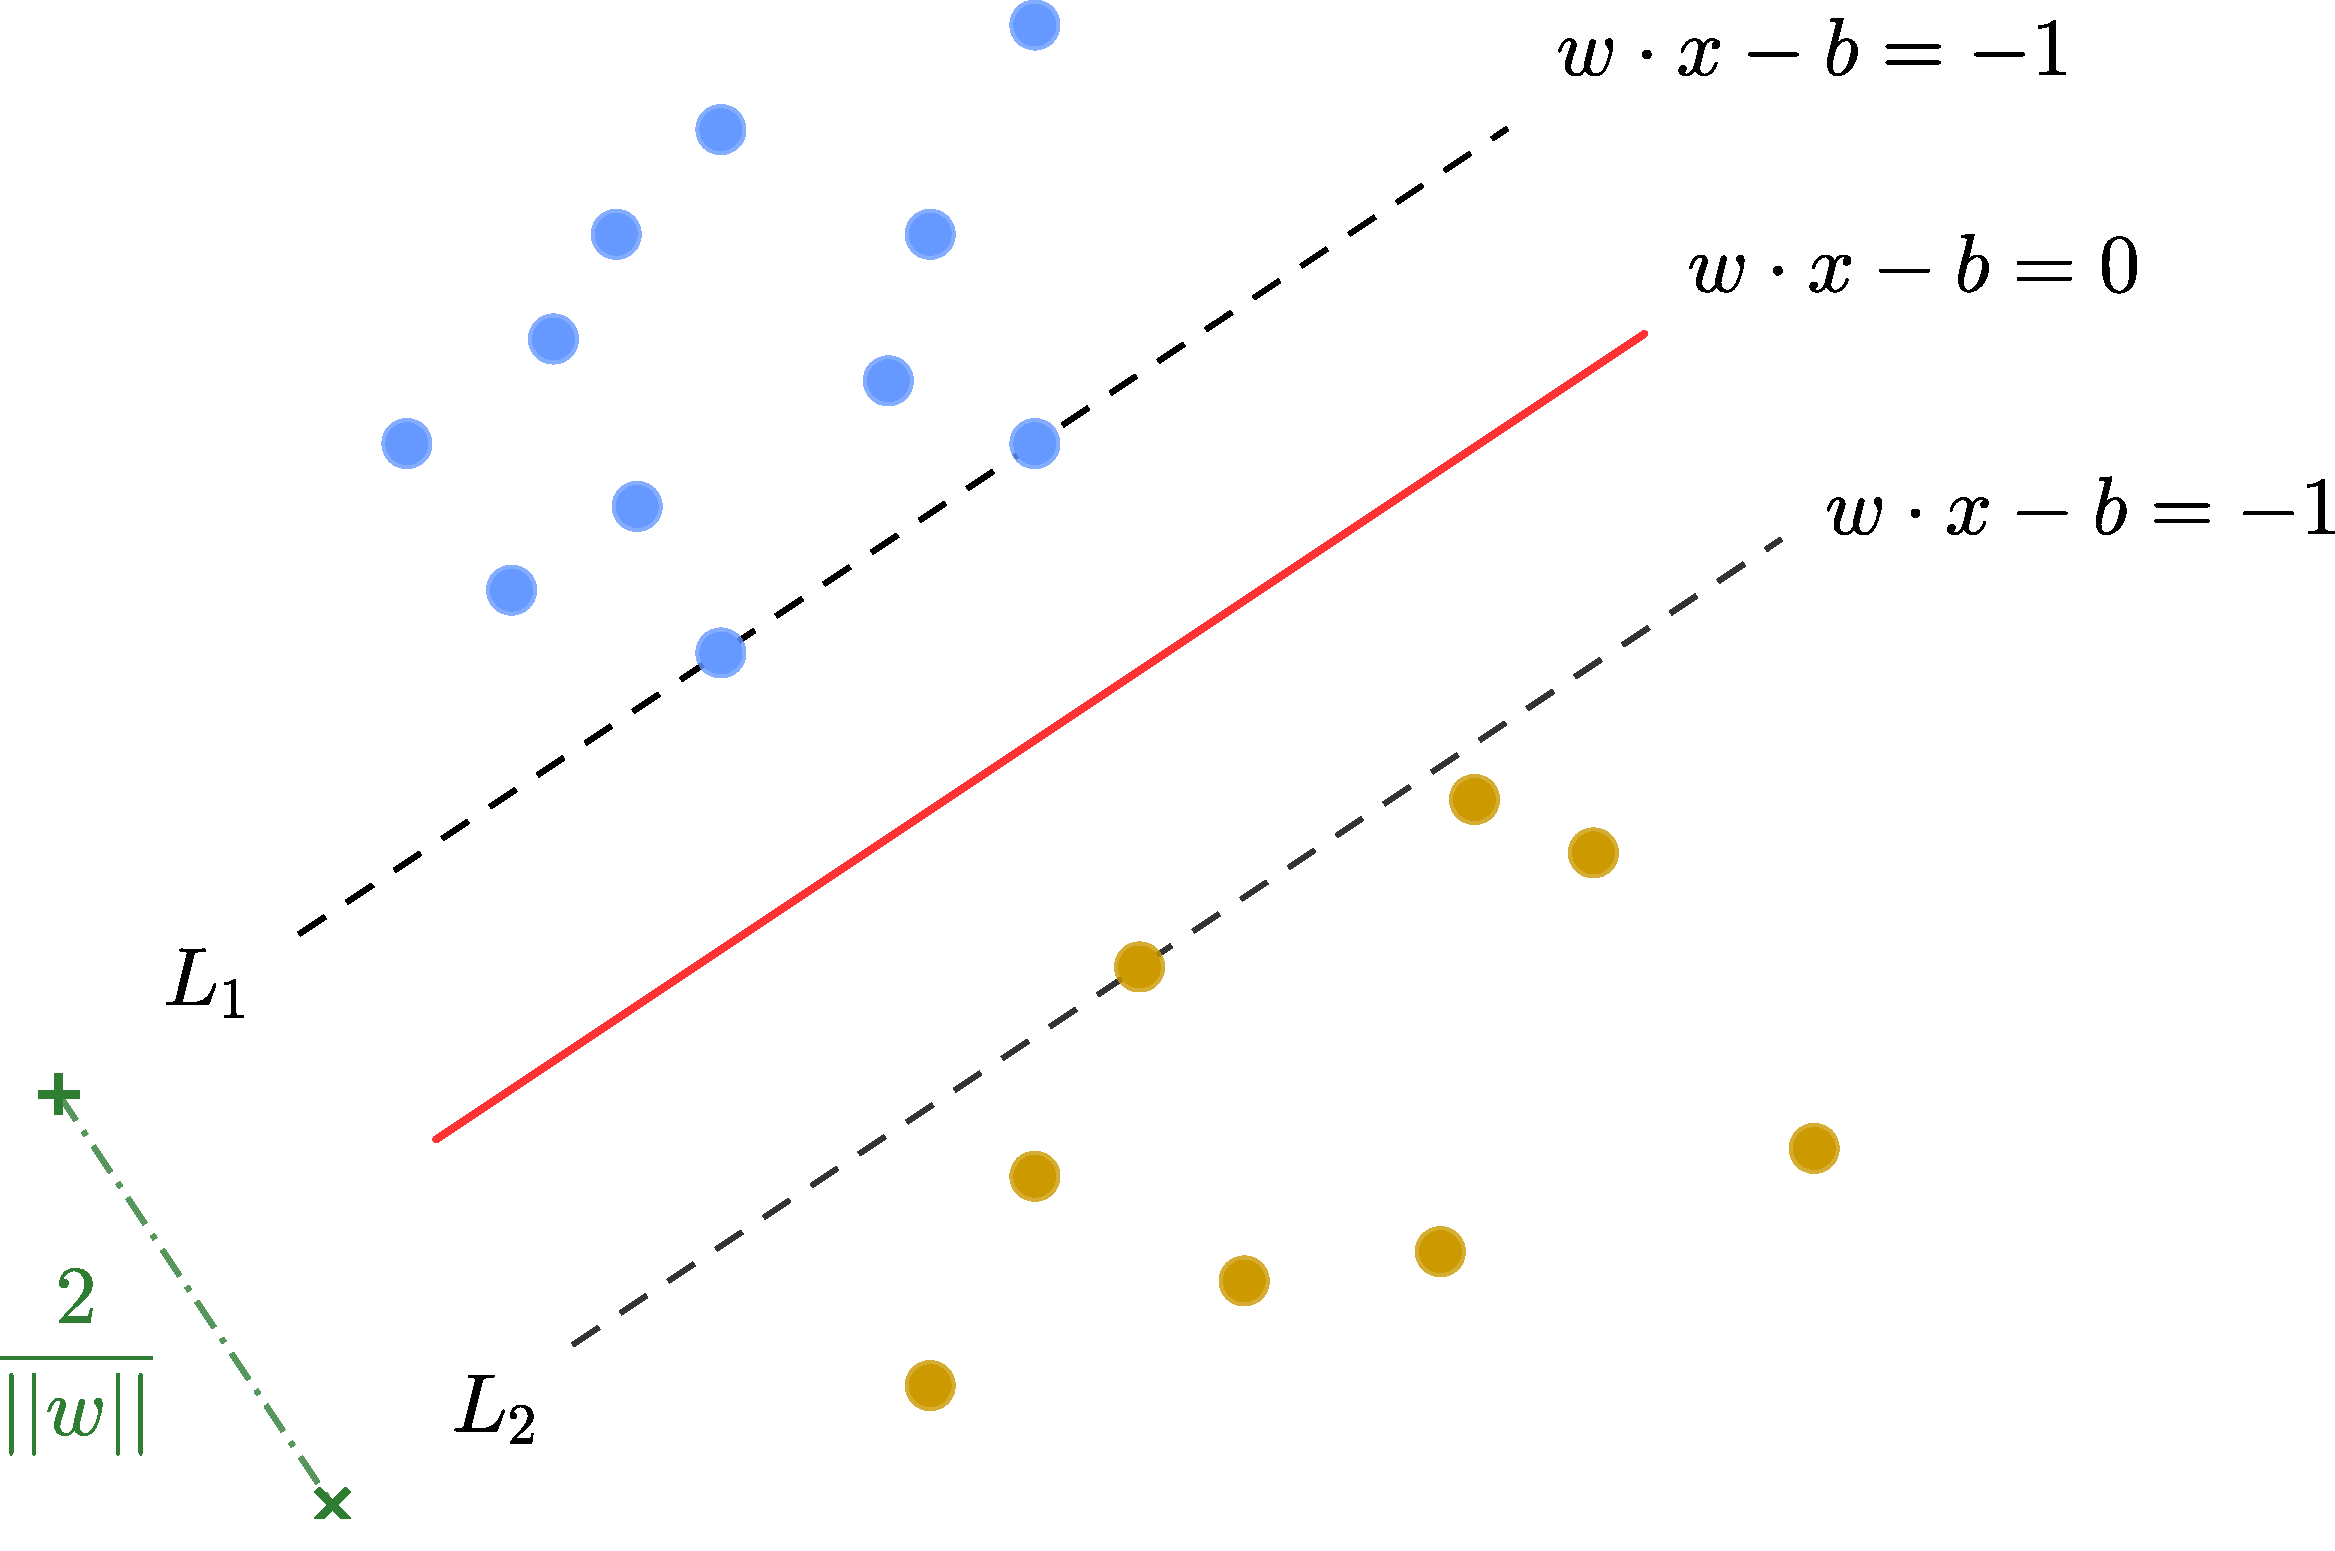
\includegraphics[width=0.8\textwidth]{Support Vector Machine}
  \caption[二維平面上最優分類線]{二維平面上最優分類線}
  \label{figure: Support Vector Machine}
\end{figure}

對於帶有限制條件的最佳化問題,通常會構造其拉格朗日函數 (Lagrange Function) 進行求解,而引入拉格朗日函數後的規劃問題在極值處必須滿足庫恩塔克條件 (Karush-Kuhn-Tucker Conditions, KKT Conditions) ;除此之外,由於線性支持向量機滿足 Slater 條件,其對偶問題將等價於原問題。因此一個線性支持向量機的對偶形式即找到一組合適的 $\boldsymbol{\alpha}$ 滿足方程式 \eqref{equation: Dual SVM Problem} 所示的最佳化問題。
%
\begin{equation}\label{equation: Dual SVM Problem}
  \begin{aligned}
    \min_{\boldsymbol{\alpha}} \qquad & \frac{1}{2} \sum_{i = 1}^{m} \sum_{j = 1}^{m} \alpha_i \alpha_j y_i y_j \boldsymbol{x}_i^{\top} \boldsymbol{x}_j - \sum_{i = 1}^{m} \alpha_{i} \\
    \text{s.t.}                \qquad & \sum_{i = 1}^{m} \alpha_{i} y_{i} = 0 \\
    \qquad                            & \alpha_{i} \geq 0 ,\quad i = 1, 2, \ldots, m
  \end{aligned}
\end{equation}
%
此時若依據庫恩塔克條件 (Karush-Kuhn-Tucker Conditions, KKT Conditions) 進行求解,所得到的最優分類函數便如方程式 \eqref{equation: SVM Function} 所示。
%
\begin{equation}\label{equation: SVM Function}
  h(\boldsymbol{x}) = \text{sgn} \left( \sum_{i \in SV}^{m} \alpha_{i}y_{i} \boldsymbol{x}_{i}^{\top} \boldsymbol{x}_{i} + b \right)
\end{equation}
%
定義支持向量 (Support Vector) 為對偶變數 $\alpha_{i} \geq 0$ 所對應的樣本,上式中的 $SV$ 即代表所有支持向量所組成的集合。

\subsubsection{核函數 (kernel Functions)}

在實際狀況中存在許多非線性可分的問題,因此不存在一個劃分超平面來將屬於不同標記的訓練樣本點進行分開,在支持向量機中透過核技巧 (kernel Trick) 將特徵空間 $\mathbb{R}^{d}$ 中非線性可分的樣本點映射至特徵空間 $\mathbb{R}^{\hat{d}}$ 中線性可分的樣本點,藉此來處理樣本非線性可分的狀況 \cite{boser1992training}。將樣本點進行適當地映射之後,支持向量機的基本型和對偶型將分別轉變為方程式 \eqref{equation: Non-Linear SVM Problem} 和方程式 \eqref{equation: Non-Linear Dual SVM Problem} 所示的最佳化問題。
%
\begin{equation}\label{equation: Non-Linear SVM Problem}
  \begin{aligned}
    \min_{\boldsymbol{w}, b} \qquad & \frac{1}{2} \boldsymbol{w}^{\top} \boldsymbol{w} \\
    \text{s.t.}              \qquad & y_{i} (\boldsymbol{w}^{\top} \boldsymbol{\phi} (\boldsymbol{x}_{i}) + b ) \geq 1 ,\quad i = 1, 2, \ldots, m
  \end{aligned}
\end{equation}
%
\begin{equation}\label{equation: Non-Linear Dual SVM Problem}
  \begin{aligned}
    \min_{\boldsymbol{\alpha}} \qquad & \frac{1}{2} \sum_{i = 1}^{m} \sum_{j = 1}^{m} \alpha_i \alpha_j y_i y_j \boldsymbol{\phi} (\boldsymbol{x}_{i})^{\top} \boldsymbol{\phi} (\boldsymbol{x}_{j}) - \sum_{i = 1}^{m} \alpha_{i} \\
    \text{s.t.}                \qquad & \sum_{i = 1}^{m} \alpha_{i} y_{i} = 0 \\
    \qquad                            & \alpha_{i} \geq 0 ,\quad i = 1, 2, \ldots, m
  \end{aligned}
\end{equation}
%
其中,$\boldsymbol{\phi} (\boldsymbol{x}_{i})$ 表示將樣本 $\boldsymbol{x}$ 映射至特徵空間 $\mathbb{R}^{\hat{d}}$ 中的特徵向量。為使計算時的複雜度降低,核技巧透過塑造一個形如方程式 \eqref{equation: Kernel Function} 所示的核函數 (Kernel Function) ,將特徵映射與內積運算壓縮為一個步驟。
%
\begin{equation}\label{equation: Kernel Function}
  \kappa (\boldsymbol{x}_{i}, \boldsymbol{x}_{j}) = \boldsymbol{\phi} (\boldsymbol{x}_{i})^{\top} \boldsymbol{\phi} (\boldsymbol{x}_{j})
\end{equation}
%
其中,核函數必須滿足 Mercer 條件 (Mercer Condition) ,亦即對於任意核函數 $\kappa (\boldsymbol{x}_{i}, \boldsymbol{x}_{j})$ 所對應的矩陣 $\boldsymbol{K} \coloneqq [\kappa (\boldsymbol{x}_{i}, \boldsymbol{x}_{j})]_{m \times m} $ 必須為半正定的 \cite{cristianini2000introduction};除此之外,核函數也可以透過現有的核函數進行線性組合得到 \cite{lanckriet2004learning}。表 \ref{table: Kernel Functions} 為滿足 Mercer 條件的常見核函數。

\begin{table}[htp]
  \centering
  \caption[滿足 Mercer 條件的常見核函數]{滿足 Mercer 條件的常見核函數}
  \begin{tabular*}{\textwidth}{ccl}
    \toprule
    \textbf{名稱}   & \textbf{形式}            & \textbf{說明}          \\
    \midrule
    線性核函數      & $\boldsymbol{x}_{i}^{\top} \boldsymbol{x}_{j}$ & 容易實現並具高解釋性,但無法解決非線 \\
    &   & 性可分問題            \\
    多項式核函數    & $\left( \beta \boldsymbol{x}_{i}^{\top} \boldsymbol{x}_{j} + \theta \right)^{n}$ & 使用維度 $n$ 來描述被映射空間複雜度,但 \\
    &   & 參數太多,當維度太大時計算較不穩定 \\
    指數徑向核函數  & $\exp \left(-\frac{\norm{\boldsymbol{x}_{i} - \boldsymbol{x}_{j}}}{2\sigma^2} \right)$ & 沒有計算不穩定的問題,但計算速度較慢 \\
    &   & 且容易過度擬合 \\
    高斯徑向核函數  & $\exp \left(-\frac{\norm{\boldsymbol{x}_{i} - \boldsymbol{x}_{j}}^2}{2\sigma^2} \right)$ & 沒有計算不穩定的問題,但計算速度較慢 \\
    &   & 且容易過度擬合 \\
    Sigmoid 核函數  & $\tanh{\left( \beta \boldsymbol{x}_{i}^{\top} \boldsymbol{x}_{j} + \theta \right)}$ & 透過支持向量機實現了神經網路,結果與 \\
    &   & 徑向核函數相似,但在某些參數下無效 \\
    \bottomrule
  \end{tabular*}
  \label{table: Kernel Functions}
\end{table}

\noindent 在實際的機器學習過程中,核函數的選擇決定了計算的性能表現、模型的合適狀況以及預測的準確程度。核函數的選取主要依靠領域背景知識進行判斷,或者是採取交叉驗證法根據不同分析情況採用不同的核函數,目前在大多數的情況下將優先採用對於任意樣本都有較好學習能力的高斯徑向核函數。

\subsubsection{支持向量迴歸 (Support Vector Regression, SVR)}

在分類問題中,支持向量機尋找一個劃分超平面將樣本點一分為二;而在迴歸問題中,支持向量機尋找的則是能夠準確預測資料分佈的平面。

假設訓練資料表示為 $\{ (\boldsymbol{x}_1, y_1), (\boldsymbol{x}_2, y_2), \ldots, (\boldsymbol{x}_{m}, y_m) \}$,其中 $\boldsymbol{x}_i$ 和 $y_i$ 分別表示第 $i$ 組資料的特徵和對應的迴歸值,且 $(\boldsymbol{x}_{i}, y_i ) \in \mathbb{R}^d \times \mathbb{R}$。支持向量迴歸能夠容忍預測值 $h(\boldsymbol{x}_i)$ 與迴歸值 $y_i$ 之間小於 $\epsilon$ 的偏差,並可以表示為方程式 \eqref{equation: Support Vector Regression} 所示的最佳化問題 \cite{drucker1997support}。
%
\begin{equation}\label{equation: Support Vector Regression}
  \begin{aligned}
    \min_{\boldsymbol{\omega}, b}   \qquad & \frac{1}{2} \norm{\boldsymbol{\omega}}^2                                                               \\
    \text{s.t.}                     \qquad & \abs{y_i - (\boldsymbol{\omega}^{\top} \boldsymbol{x_i} + b)} \leq \epsilon ,\quad i = 1, 2, \ldots, m
  \end{aligned}
\end{equation}
%
同樣地,在構造其拉格朗日函數並使用核函數將非線性可分的訓練資料進行映射後,支持向量迴歸可以形式化為方程式 \eqref{equation: Support Vector Regression Model} 所示的最佳化模型。
%
\begin{equation}\label{equation: Support Vector Regression Model}
  \begin{aligned}
    \min_{\boldsymbol{\omega}, b}   \qquad & \frac{1}{m} \sum_{i = 1}^{m} \max{\left(0, \abs{y_i - (\boldsymbol{\omega}^{\top} \boldsymbol{\phi}(\boldsymbol{x}_i) + b)} - \epsilon \right)} + \frac{\lambda}{2} \boldsymbol{\omega}^{\top}\boldsymbol{\omega}
  \end{aligned}
\end{equation}

\subsection{模型評價方法}

我們通常透過計算預測結果與實際數據之間的誤差,來作為比較不同預測模型的評價指標,本研究將採用文獻上常見三種預測評估指標作為模型評價標準,分別是:(1) 平均絕對誤差 (Mean Absolute Error, MAE) 、平均絕對百分比誤差 (Mean Absolute Percentage Error, MAPE) 與均方根誤差 (Root Mean Squares Error, RMSE) 。以下分別介紹這些方法:

\subsubsection{平均絕對誤差 (Mean Absolute Error, MAE)}

平均絕對誤差即將每筆預測值與實際值的絕對殘差值進行平均,可以用來檢視預測結果的誤差範圍,屬於絕對指標值,其計算方式如式 \eqref{equation: MAE} 所示:
%
\begin{equation} \label{equation: MAE}
  E_{\text{MAE}} = \frac{1}{n} \sum_{i = 1}^{n} \abs{\hat{y}_{i} - y_i}
\end{equation}
%
其中,$n$ 為樣本數;$\hat{y_i}$ 為第 $i$ 項的估計值,$y_i$ 為第 $i$ 項的實際值。其缺點為沒有考慮實際值的平均數,因此無法單純由其數值判斷結果的好壞,需與其他預測模型進行比較。

\subsubsection{平均絕對百分比誤差 (Mean Absolute Percentage Error, MAPE)}

平均絕對百分比誤差又稱為平均絕對誤差率,為每筆預測值與實際值的絕對誤差值除以實際值之和,為誤差百分率的平均值,可以用來評估預測模型準確程度的指標,屬於相對指標值,其計算方式如式 \eqref{equation: MAPE} 所示:
%
\begin{equation} \label{equation: MAPE}
  E_{\text{MAPE}} = \frac{1}{n} \sum_{i = 1}^{n} \abs{\frac{\hat{y}_{i} - y_i}{y_i}} \times 100\%
\end{equation}
%
其中,$n$ 為樣本數;$\hat{y_i}$ 為第 $i$ 項的估計值,$y_i$ 為第 $i$ 項的實際值。此值若越接近 $0$ 則表示預測效果越好,值得注意的是實際值中若出現數值為 $0$ 之狀況將會導致無法計算結果。

\subsubsection{均方根誤差 (Root Mean Squares Error, RMSE)}

均方根誤差亦稱為標準誤差,為每筆預測誤差平方和的平均值方根,可以用來了解預測模型的可靠程度,屬於相對指標值,其計算方式如式 \eqref{equation: RMSE} 所示:
%
\begin{equation} \label{equation: RMSE}
  E_{\text{RMSE}} = \sqrt{\frac{1}{n} \sum_{i = 1}^{n} (\hat{y}_{i} - y_i)^2}
\end{equation}
%
其中,$n$ 為樣本數;$\hat{y_i}$ 為第 $i$ 項的估計值,$y_i$ 為第 $i$ 項的實際值。其特性為對特大或特小的誤差較為敏感,能夠反映出預測過程中的精密程度,但同時由於單位和大小與實際值不同,無法用以評斷預測值和實際值之間的差距。

% \begin{enumerate}
% %   \item \textbf{均方誤差 (Mean Square Error, MSE)}:
% %         \begin{equation} \label{equation: MSE}
% %           E_{\text{MSE}} = \frac{1}{n} \sum_{i = 1}^{n} (\hat{y}_{i} - y_i)^2
% %         \end{equation}
%   \item \textbf{均方根誤差 (Root Mean Squares Error, RMSE)}:
%         \begin{equation} \label{equation: RMSE}
%           E_{\text{RMSE}} = \sqrt{\frac{1}{n} \sum_{i = 1}^{n} (\hat{y}_{i} - y_i)^2}
%         \end{equation}
%   \item \textbf{平均絕對誤差 (Mean Absolute Error, MAE)}:
%         \begin{equation} \label{equation: MAE}
%           E_{\text{MAE}} = \frac{1}{n} \sum_{i = 1}^{n} \abs{\hat{y}_{i} - y_i}
%         \end{equation}
%   \item \textbf{平均絕對百分比誤差 (Mean Absolute Percentage Error, MAPE)}:
%         \begin{equation} \label{equation: MAPE}
%           E_{\text{MAPE}} = \frac{100 \%}{n} \sum_{i = 1}^{n} \abs{\frac{\hat{y}_{i} - y_i}{y_i}}
%         \end{equation}
% \end{enumerate}

\section{收益模型分析}

\subsection{自由電力市場}

早期世界各國的電力供應具有壟斷特性,直至二十世紀末歐美各國才紛紛重新組織電力產業,打破垂直整合的獨佔電力市場。自由電力市場會使得電力價格由市場機制決定,良性競爭將迫使電價下跌並推動電力設備升級,使用者也因此能受到更加專業與透明的電力服務。

\subsubsection{電力市場架構}

\begin{figure}
  \centering
  \begin{subfigure}[b]{0.475\textwidth}
    \centering
    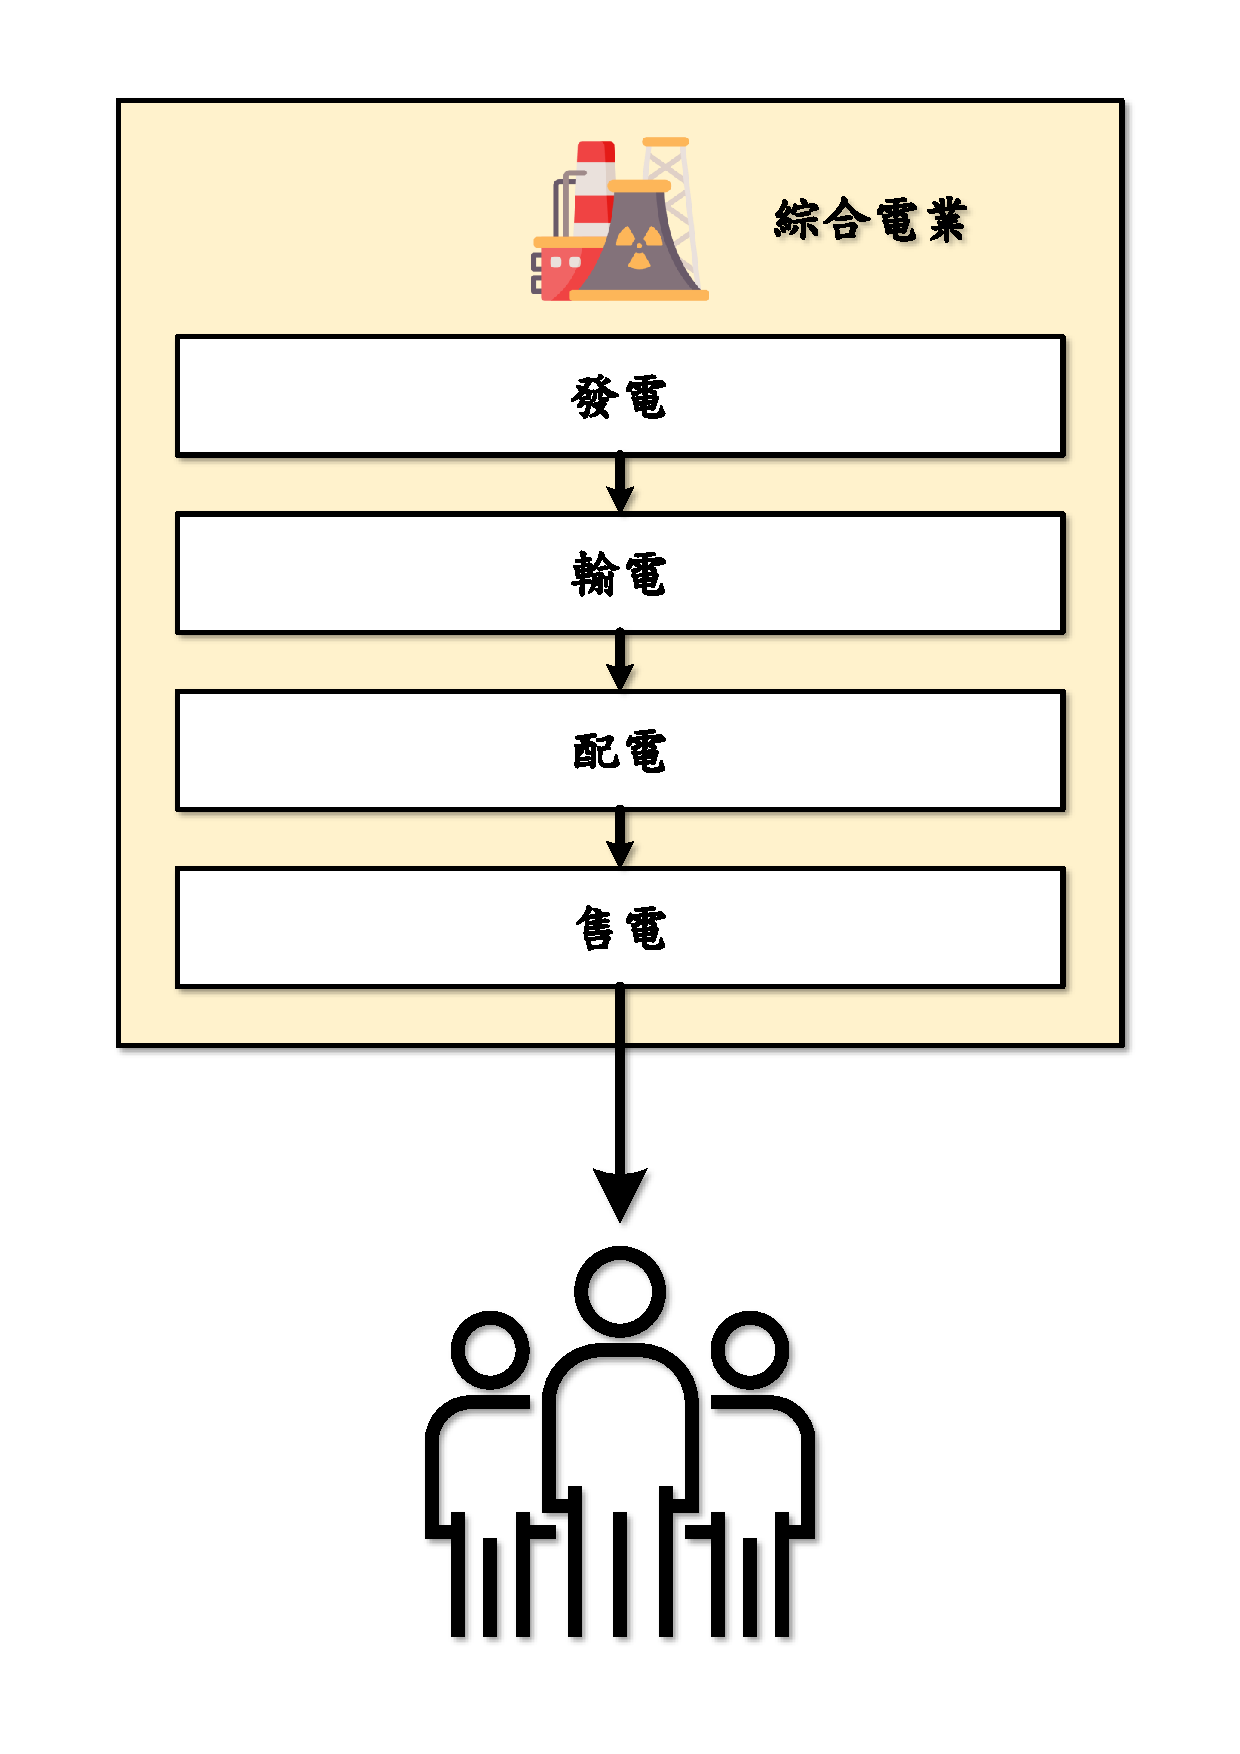
\includegraphics[width=\textwidth]{Power Monopoly Market}
    \caption[垂直壟斷]{垂直壟斷}
  \end{subfigure}
  \hfill
  \begin{subfigure}[b]{0.475\textwidth}
    \centering
    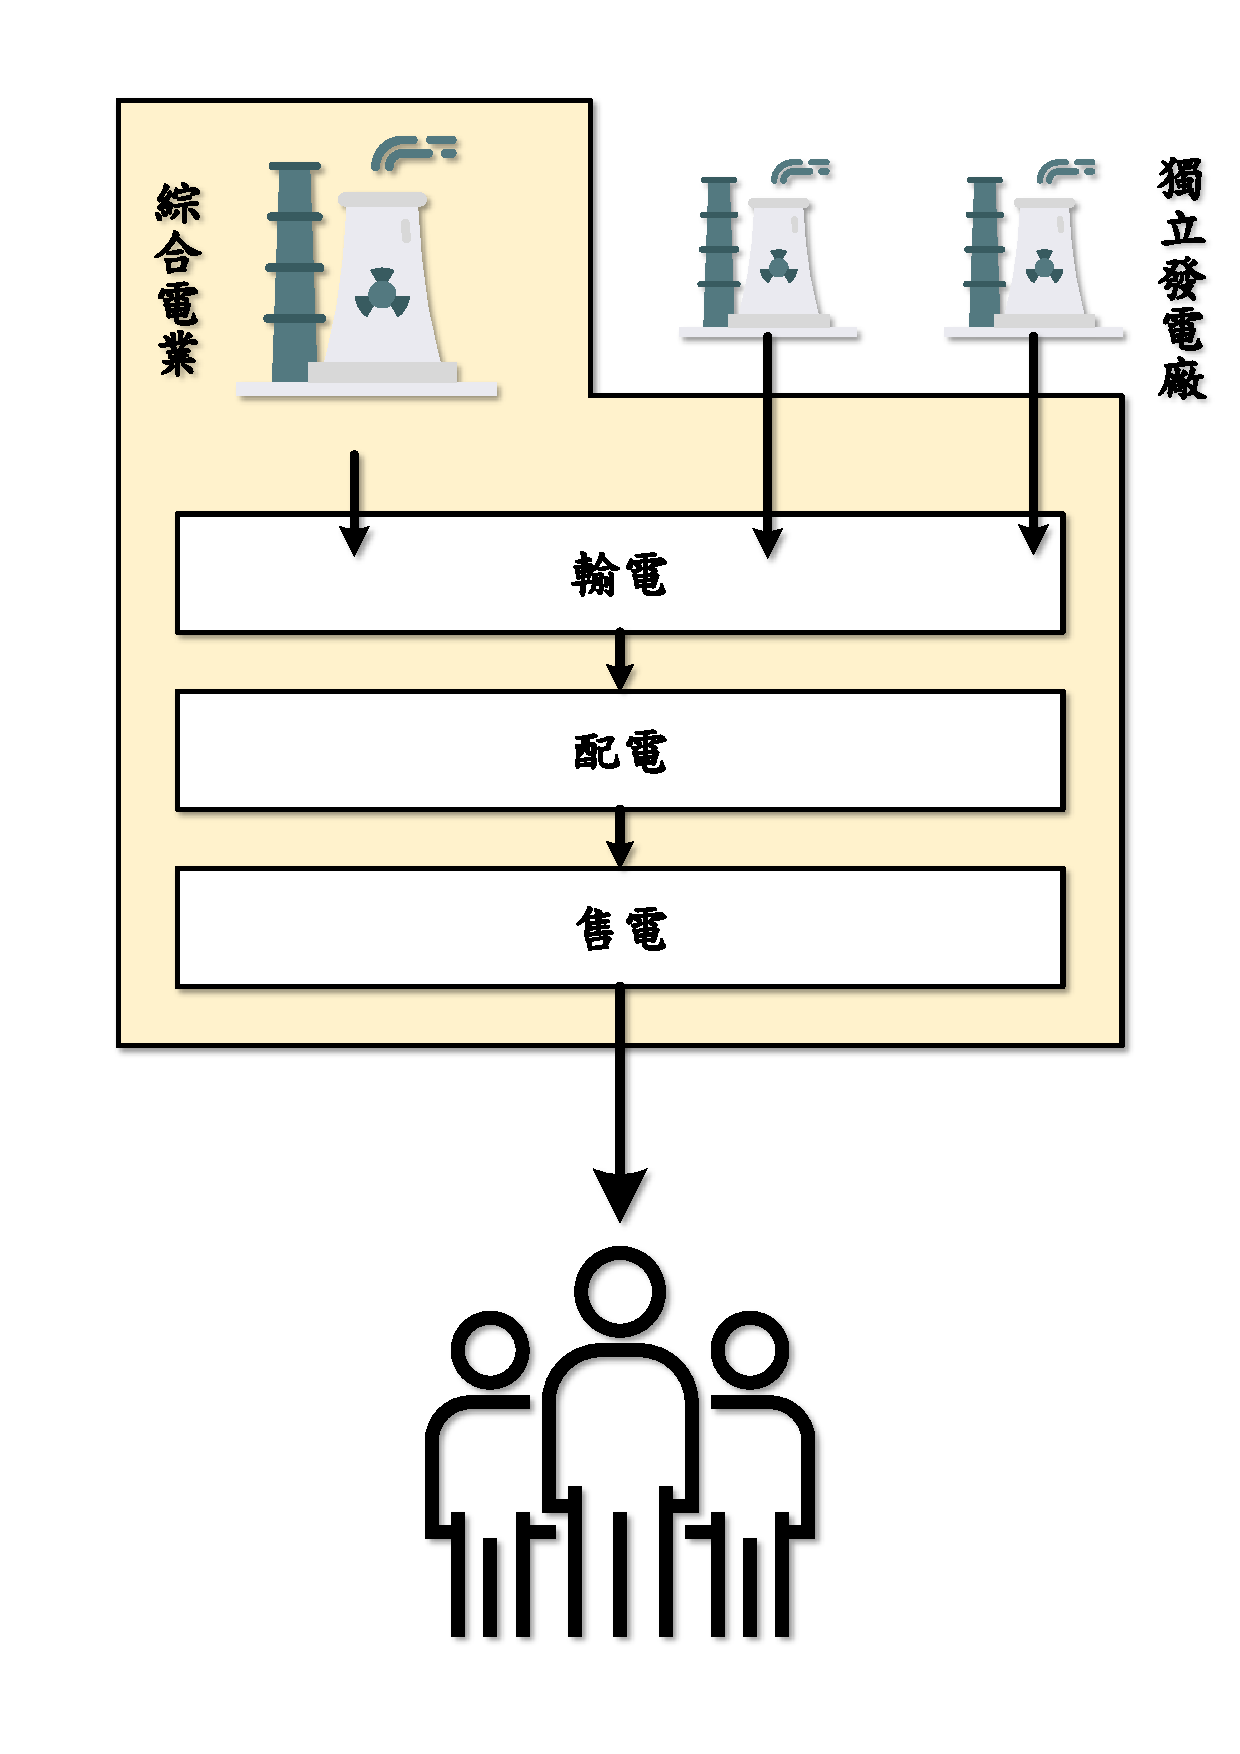
\includegraphics[width=\textwidth]{Power One-Buy Market}
    \caption[單一買方]{單一買方}
  \end{subfigure}
  \hfill
  \begin{subfigure}[c]{0.475\textwidth}
    \centering
    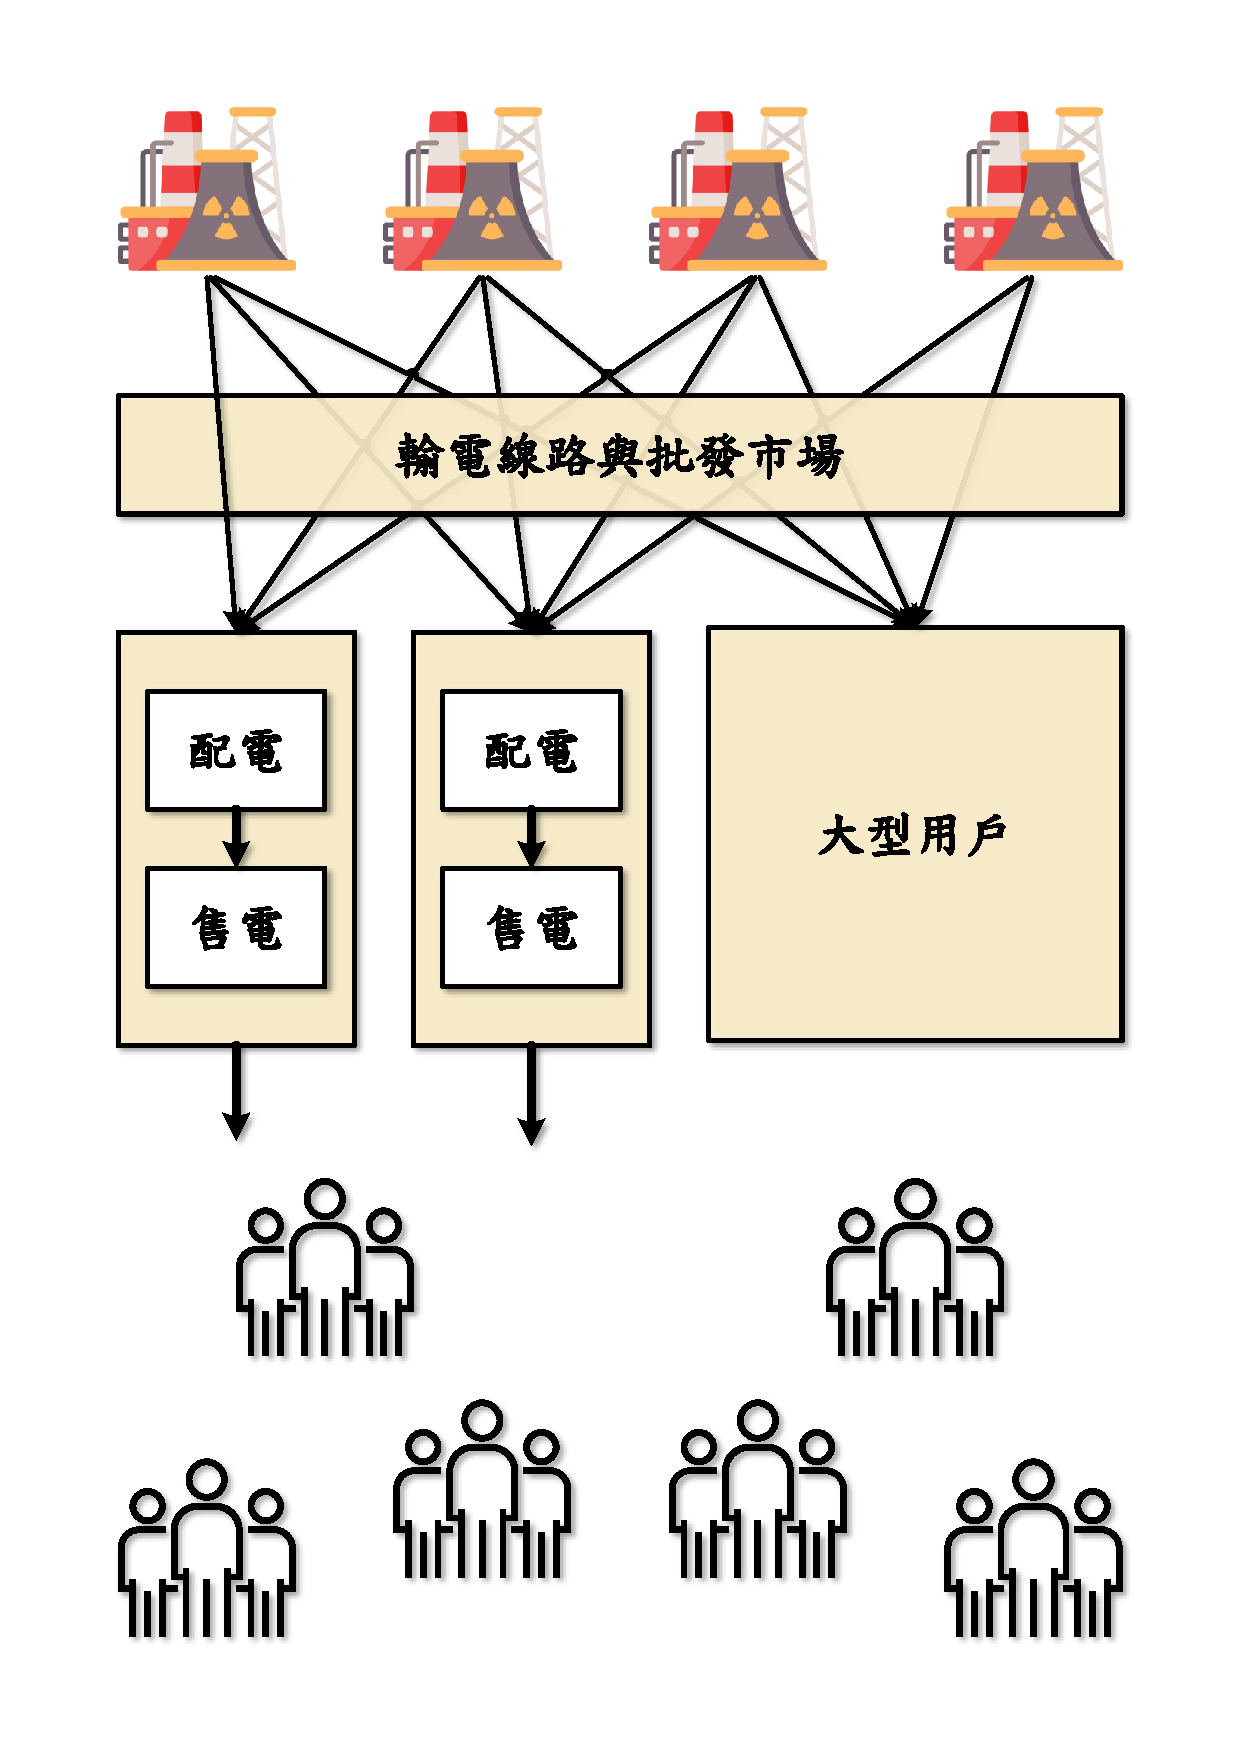
\includegraphics[width=\textwidth]{Power Wholesale Market}
    \caption[批發競爭]{批發競爭}
  \end{subfigure}
  \hfill
  \begin{subfigure}[d]{0.475\textwidth}
    \centering
    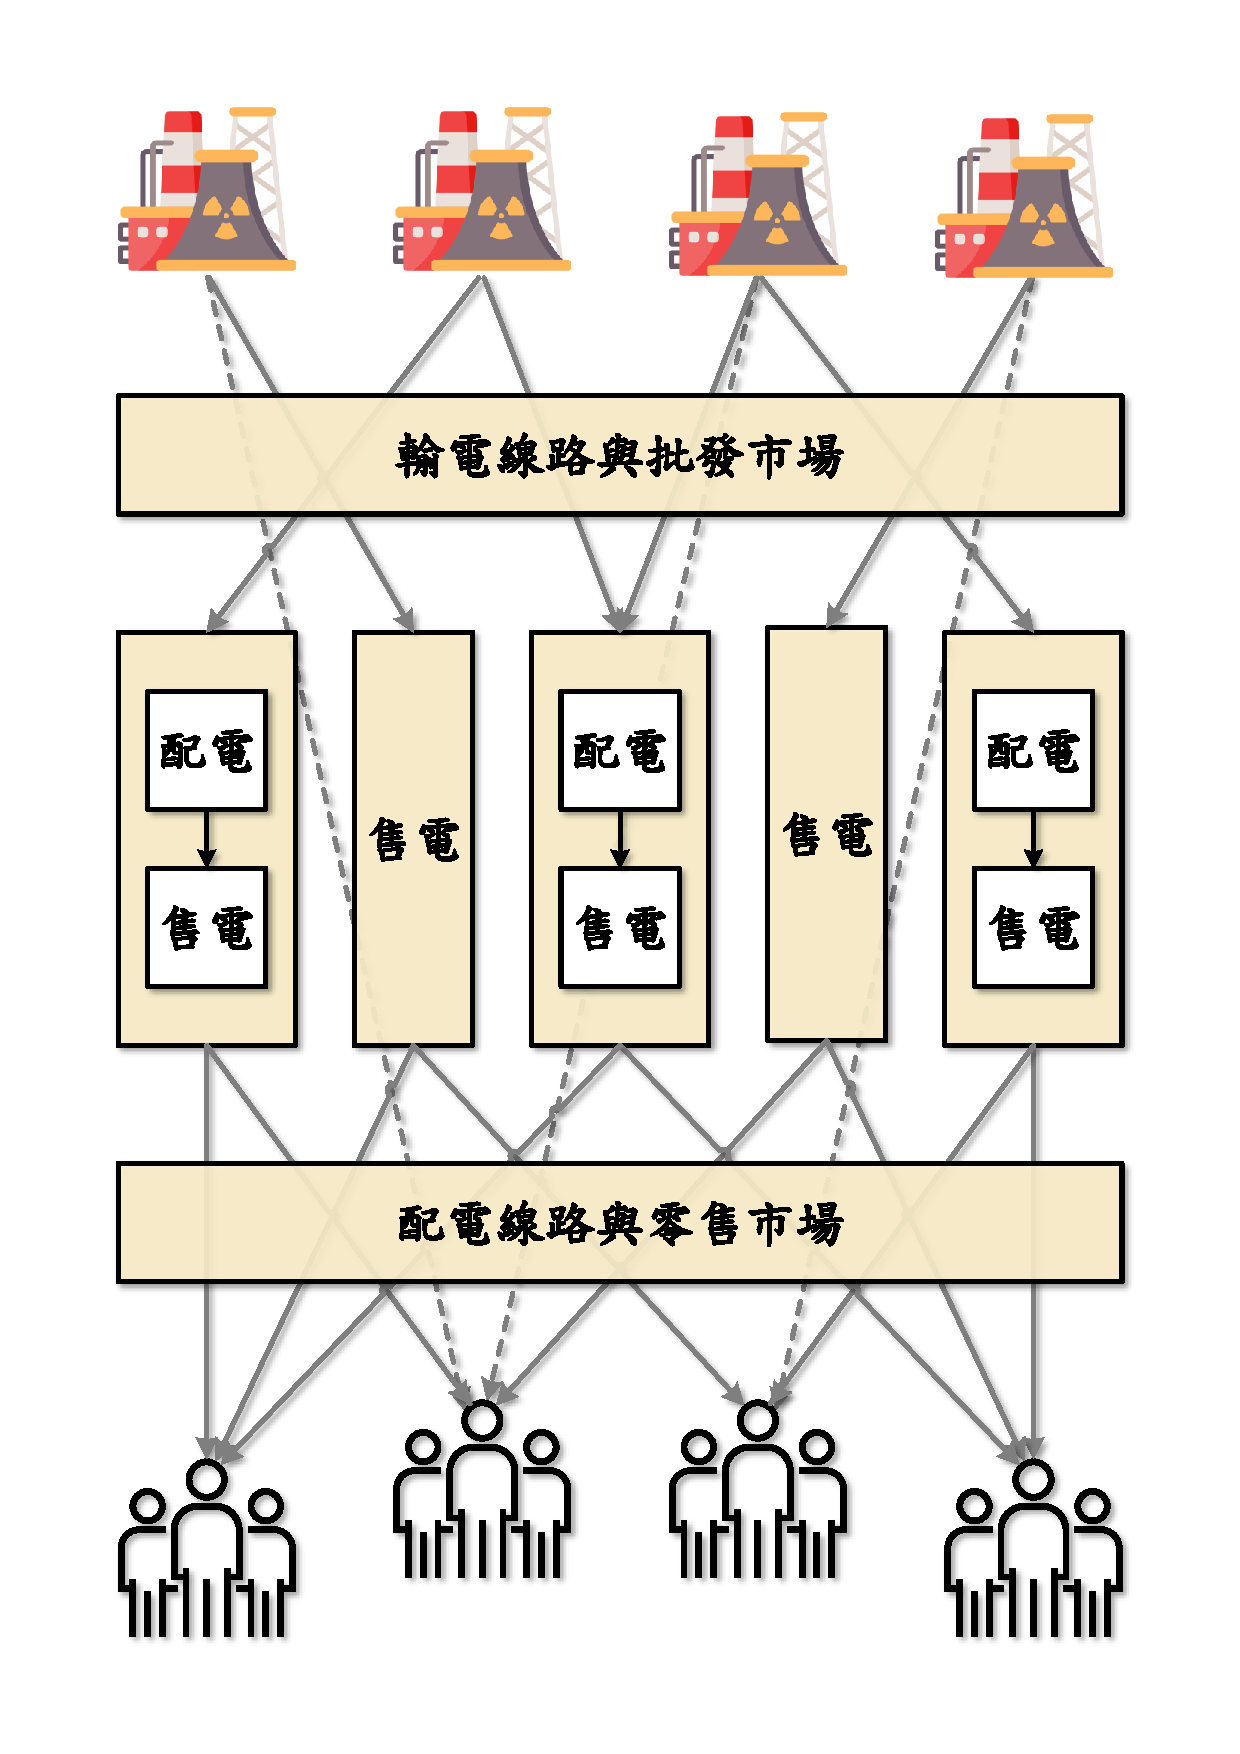
\includegraphics[width=\textwidth]{Power Retail Market}
    \caption[零售競爭]{零售競爭}
  \end{subfigure}
  \hfill
  \caption[常見電力市場架構]{常見電力市場架構}
  \label{figure: Power Markets}
\end{figure}

國際上電力市場的發展歷程,主要可以將電力市場分成垂直壟斷、單一買方、批發競爭及零售競爭等四個主要架構,如圖 \ref{figure: Power Markets} 所示 \cite{wang2015powermarket}。在獨佔電力市場中,由一家獨佔電力機構將上下游所有的發電、輸電、配電與售電業務進行垂直整合;而在自由電力市場中,則將上下游所有的發電、輸電、配電與售電業務水平分割成能夠獨立運作的機構 \cite{shahidehpour2003market},這些機構可能為:

\begin{itemize}
  \item \textbf{能源供應商 (Generation Company, GENCO)}:電力市場中的供給端,調度可支配的發電機組生產能源,並根據簽訂的售電合約或電力拍賣進行出售。可以藉由調度發電機組和選擇不同交易方式來調整自身收益狀況。
  \item \textbf{電力使用者 (Customer)}:電力市場中的需求端,獨佔電力市場中只能任由垂直整合綜合電業的電力公司制定電價進行交易,自由電力市場中可以自由選擇實惠的能源供應商簽約。通常根據規模可以分為大型用戶和個體用戶,大型用戶可以買賣電力,個體用戶僅能進行電力消費。
  \item \textbf{電力調度中心 (Independent System Operator, ISO)}:負責制定市場運作規則、發電調度控制、維持系統安全,並以絕對中立的方式提供使用者進行交易。
\end{itemize}

\subsubsection{市場交易方式}

綜合目前世界上已實施電業自由化之各國的電力買賣方式,依據交易地點的分散與否,可以將自由化電力市場的交易方式分成以下三種 \cite{li2005strategic}:
%
\begin{itemize}
  \item \textbf{雙邊合約模式 (Bilateral Contract Model)}:由供給端的能源供應商與需求端的電力使用者雙方直接簽訂交易合約,明定在特定時間內所願意交易的價格與數量,由電力調度所負責制定合約規範並在運作過程中檢驗供電品質。此模式下的供需雙方擁有較多選擇,但可能存在資訊不對等的狀況。
  \item \textbf{電力池模式 (PoolCo Model)}:供給端的能源供應商與需求端的電力使用者必須向公正的電力交易場所 (Power Exchange, PX) 提出電力需求與競標價格,電力交易場所將依據雙方提供的資訊訂定市場結清價格 (Market-Clearing Price) 並告知買賣雙方進行交易。此模式下的供需雙方沒有太多選擇,但集中的協調、調度與定價流程有利於市場競爭。
  \item \textbf{混合型模式 (Hybrid Model)}:結合了雙邊合約模式與電力池模式,供給端的能源供應商和需求端的電力使用者可以直接簽訂交易合約,也可以向電力交易所提出電力需求與競標價格,並從中選擇對自己較為有利的交易方式。此模式下既保留了一定的公平性,亦提供了相當程度的選擇。
\end{itemize}
%
其中,採用電力池模式或混合型模式的電力市場,皆需要透過電力交易場所 (Power Exchange, PX) 進行競標。目前根據電力調度中心與電力交易場所排程運作的時間,自由電力市場可以分成長期的期貨市場 (Future Market) 與短期的現貨市場 (Spot Market) 。電力期貨市場可以進行跨幅提前數週、數月甚至數年的電力交易,以避免未來可能的價格波動;電力現貨市場包括了日前市場 (Day-Ahead Market) 、日內市場 (Intraday Market) 與即時市場 (Real-Time Market) ,其中又以日前市場最為常見。

在日前市場中,電力調度中心將於調度能源的前一天在電力交易場所公告預測的電力需求、電力最高價格、電力最低價格與競標重複一次所需時間等相關交易資料,市場參與者必須在限定時間內提交可供調度的電力供給與競標價格,最後自最低的價格開始進行調度直至滿足前一日預測的電力需求為止。

\subsection{風機功率模型}

風力發電的原理,是借助風力推動風機轉動葉片,透過齒輪箱提升轉速後經由發電機進行發電,其中涉及了一系列風能、機械能與電能的轉換過程。本研究中採用風力發電機組的標準功率曲線作為風機模型,用以將風速轉換為對應的風能。風速與功率的對應關係一般以分段函數表示如方程式 \eqref{equation: Wind Power Model} 所示:
%
\begin{equation}\label{equation: Wind Power Model}
  p_{\text{wt}}(v) = \left\{
  \begin{array}{cl}
    \displaystyle p_{\text{r}} \cdot \frac{v^{3} - v_{\text{in}}^{3}}{v_{\text{r}}^{3} - v_{\text{in}}^{3}} & ,~ {v}_{\text{in}} < v < v_{\text{r}} \\[0.5em]
    p_{\text{r}} & ,~ v_{\text{r}} \leq v < v_{\text{out}} \\[0.5em]
    0 & ,~ \text{otherwise}
  \end{array}\right.
\end{equation}
%
其中,$P_{\text{wt}}(v)$ 為風力發電機組在風速為 $v$ 時所輸出的功率;$p_{\text{r}}$ 為風力發電機組的額定功率,又稱為裝置容量 (capacity) ,亦即風力發電機組所能輸出的最大功率;$v_{\text{in}}$ 為風力發電機組的啟動風速,又稱為切入風速 (cut-in speed) ,當風速大於啟動風速才開始運轉;$v_{\text{out}}$ 為風力發電機組的停機風速,又稱為切出風速 (cut-out speed) ,當風速大於停機風速時會因安全考量停止自動運轉;$v_{\text{r}}$ 為風力發電機組的額定風速 (rated speed) 。

方程式 \eqref{equation: Wind Power Model} 表示:當風力發電機組的輸入風速大於啟動風速時,風力發電機組開始運轉,並根據不同的輸入風速產生相對應的電能,當風速達到額定風速時將以額定輸出功率運轉,當風速超過停機風速時,為保護葉片而停止輸出功率。

\subsection{電動汽車電池}

電動汽車係透過電池儲能的輸出推動馬達來行駛,為使電動汽車參與虛擬電廠進行電力市場交易,需要針對電動汽車電池原理進行了解。

\subsubsection{電池設備概述}

儲能電池設備透過電池內部的化學反應進行能量的釋放與儲存,一般儲能電池用於在緊急斷電狀況下及時供電或在用電尖峰時刻穩定電力系統,而電動汽車儲能電池為了推動馬達,還需要具備能夠長時間輸出一定大小電流。儲能電池設備主要由電池管理系統、交流/直流雙向轉換器與電池組所構成 \cite{qian2010high}。

其中車用電池管理系統需要針對電池充電狀況 (State of Charge, SOC) 與電池健康狀況 (State of Health, SOH) 進行評估與建模;交流/直流雙向轉換器與充電座進行能量轉移,用於將電池輸出的直流電轉換為交流電或將交流充電座輸入的交流電轉換為直流電;電池組則由多個電池串聯組成,電動汽車主要採用二次電池作為動力來源,約略可以分為鉛酸電池、鎳鎘電池、鎳氫電池與鋰離子電池,表 \ref{table: EV Battery} 為常見二次電池的特性比較 \cite{hsu2009evbattery},目前由於鋰電池相較其他電池而言具有較大的電流輸出與安全性,因此目前電動汽車廠商多針對鋰電池進行研究與推行車款。

\begin{table}[htbp]
  \centering
  \caption[常見二次電池的特性比較]{常見二次電池的特性比較}
  \begin{tabular*}{\textwidth}{lccccc}
    \toprule
    & \textbf{鉛酸電池} & \textbf{聶鎘電池} & \textbf{鎳氫電池} & \textbf{鋰錳電池} & \textbf{磷酸鋰電池} \\
    \midrule
    \textbf{工作電壓} (V) & $2$ & $1.2$ & $1.2$ & $3.7$ & $3.3$ \\
    \textbf{體積能量密度} (\si{\Wh}/L) & $100$ & $150$ & $250$ & $285$ & $270$ \\
    \textbf{重量能量密度} (\si{\Wh}/\si{\kg}) & $30$ & $60$ & $80$ & $110$ & $120$ \\
    \textbf{電池功率密度} (\si{\Wh}/\si{\kg}) & $300$ & $150$ & $800$ & $400$ & $2000$ \\
    \textbf{循環壽命} (次) & $400$ & $500$ & $500$ & $> 500$ & $> 2000$ \\
    \textbf{能量效率} (\%) & $60\%$ & $75\%$  & $70\%$ & $90\%$ & $95\%$ \\
    \textbf{安全性} & 佳 & 佳 & 佳 & 尚可 & 優 \\
    \textbf{充電時間} & 長 & 短 & 中 & 中 & 短 \\
    \textbf{記憶效應} & 無 & 大 & 小 & 無 & 無 \\
    \textbf{環保問題} & 有 & 有 & 無 & 無 & 無 \\
    \bottomrule
  \end{tabular*}
  \label{table: EV Battery}
\end{table}

\subsubsection{電池充電方法}

電池壽命除了會隨循環使用次數增加而降低之外,亦受到電池的充電與放電方式影響,採用適合的充電方法對於保護電池十分重要,常見的基本充電方法有定電壓充電法 (Constant Voltage Charge) 、定電流充電法 (Constant Current Charge) 與脈衝充電法 (Pulsed Charge) 。其中定電壓充電法為最普遍的充電方式,但存在無法確切估計充電時間且充電初期電流較大的問題;定電流充電法根據充電時間與電池容量設定電流值,但並未考慮初始電量狀態,充電效率不高且在高電壓時電池溫度會急遽上升;脈衝充電法透過週期性電流進行充電,能適當調整電流大小並有時間予以緩衝。

電池使用過程中,輸出容量佔其額定容量 $E$ ($\text{Ah}$) 的百分比稱為放電深度 (Depth of Discharge, DoD) ,定義如方程式 \eqref{equation: Depth of Discharge} 所示,其中 $E$ ($\text{Ah}$) 為電池額定容量,$E_{r}$ ($\text{Ah}$)  為電池剩餘電量。
%
\begin{equation}\label{equation: Depth of Discharge}
  \text{DoD}~(\%) = \frac{E - E_{r}}{E} \times 100 \%
\end{equation}
%
不同的放電深度會影響二次電池的充電放電循環次數 \cite{dogger2010characterization},因此一般會將電池壽命以其生命週期內的放電次數函數 $L(\text{DoD})$ 進行表示。

\subsection{模型預測控制}

模型預測控制 (Model Predictive Control, MPC) ,又稱為移動時域控制 (Moving Horizon Control, MHC) 或後退時域控制 (Receding Horizon Control, RHC) ,是在自動控制領域中被廣泛應用於工業上的一種反饋控制策略 \cite{richalet1978model}。透過模型預測控制可以在每一個時刻都根據當前的資訊求解有限時域內的最佳化問題,因此能夠更加精準地進行系統的控制,相較於傳統的控制方法更適合用於複雜系統中。

\subsubsection{模型預測控制基本原理}

模型預測控制的基本原理如圖 \ref{figure: Model Predictive Contrl} 所示,左側為過去時刻的狀態,右側為未來時刻的狀態。模型預測控制法在當前時刻 $k$ 時, 根據過去時刻的狀態進行最佳化求解並預測未來輸出結果,在下一時刻時取前一次所得到的預測結果並捨棄其餘結果,並反覆進行此過程。一般而言,可以將模型預測控制的實現步驟依序拆解為模型預測、滾動優化與反饋校正三個部分:

\begin{figure}[htbp]
  \centering
  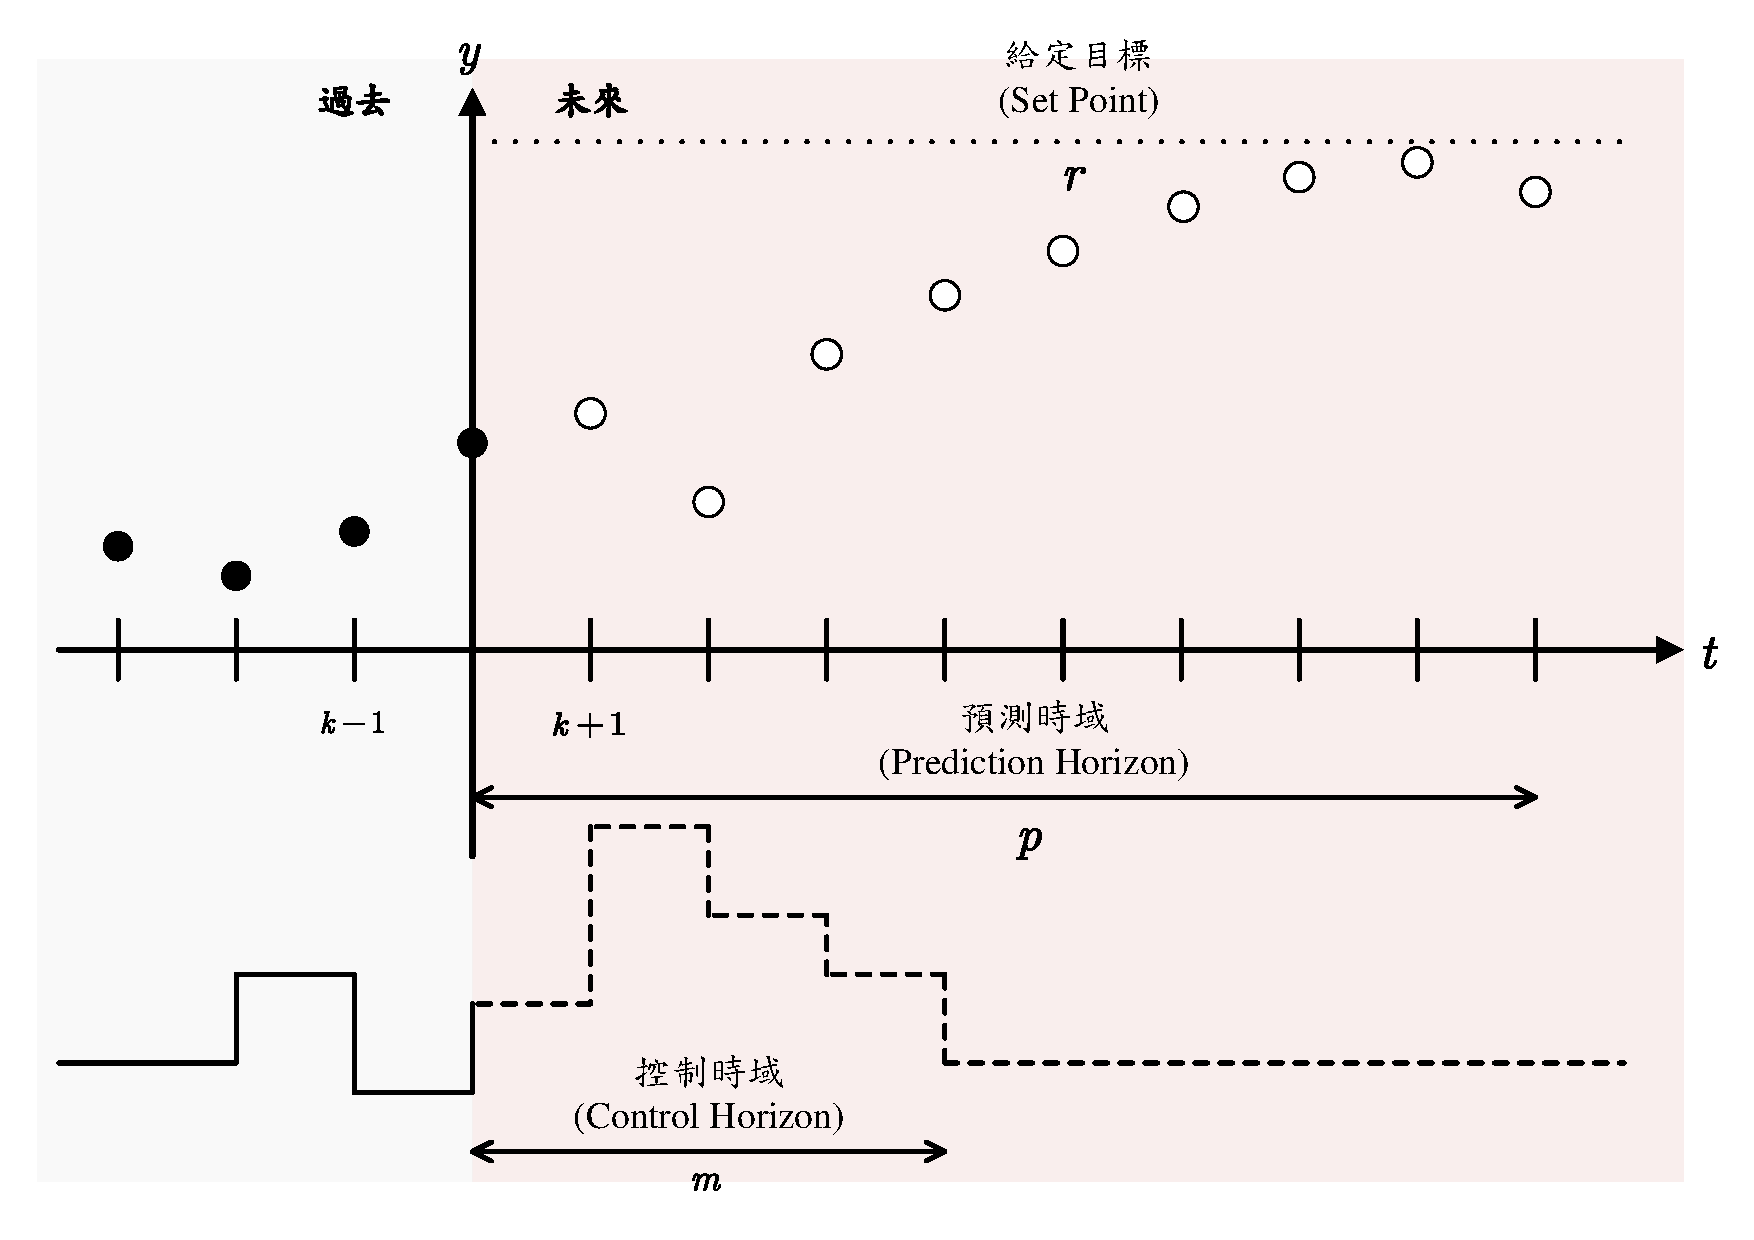
\includegraphics[width=\textwidth]{Model Predictive Control}
  \caption{模型預測控制基本原理}
  \label{figure: Model Predictive Contrl}
\end{figure}

\begin{enumerate}[label = (\arabic*)]
  \item \textbf{模型預測}:此部分為模型預測控制的基礎,根據系統的當前狀態和預測模型,對未來行為與輸出進行預測,其中預測模型通常以狀態方程式的形式表示
  \item \textbf{滾動優化}:模型預測控制在未來的有限時域內,透過某一性能指標的參考值進行未來控制決策的最佳化,其中下一時刻的只使用當前所得到控制變數來進行最佳化,並且反覆進行這個過程
  \item \textbf{反饋校正}:由於採用有限時域進行預測,封閉的控制系統中同時存在外部干擾與內部模型不確定性,每一時刻都需要檢測當前系統實際的狀況,並根據實際數值與預測結果之間的誤差進行校正
\end{enumerate}

\subsubsection{模型預測控制數學模型}

考慮線性離散時間系統的狀態空間模型如方程式 \eqref{equation: Linear Discrete System State Model} 所示:
%
\begin{equation}\label{equation: Linear Discrete System State Model}
  \begin{aligned}
    x(k + 1)  & = Ax(k) + B_{u} u(k) + B_{d} d(k) \\
    y_{c} (k) & = C_{c} x(k)                      \\
    y_{b} (k) & = C_{b} x(k)
  \end{aligned}
\end{equation}
%
其中,$k$ 為當前時刻,$x(k) \in \mathbb{R}^{n}$ 為狀態變數,$u(k) \in \mathbb{R}^{n}$ 為控制變數,$y_{c}(k) \in \mathbb{R}^{n}$ 和 $y_{b} (k) \in \mathbb{R}^{n}$ 為被控輸出變數與約束輸出變數,$d(k) \in \mathbb{R}^{n}$ 為可以被測量的外部干擾變數,而 $A, B_{u}, B_{d}, C_{c}$ 和 $C_{b}$ 為對應維度大小的系統矩陣。方程式 \eqref{equation: Linear Discrete System State Model} 表示下一時刻的狀態變數 $x(k + 1)$ 可以由當前時刻的狀態變數 $x(k)$ 和控制變數 $u(k)$ 進行預測,且輸出變數為狀態變數與控制變數的函數。

為減少與消除靜態誤差,考慮方程式 \eqref{equation: Linear Discrete System State Model Argument} 所示的增量模型:
%
\begin{equation}\label{equation: Linear Discrete System State Model Argument}
  \begin{aligned}
    \Delta x(k + 1) & = A \Delta x(k) + B_{u} \Delta u(k) + B_{d} \Delta d(k) \\
    y_{c} (k)       & = C_{c} \Delta x(k) + y_{c} (k-1)                       \\
    y_{b} (k)       & = C_{b} \Delta x(k) + y_{b} (k-1)
  \end{aligned}
\end{equation}
%
其中,$\Delta x(k) = x(k) - x(k-1)$ 為狀態增量,$\Delta u(k) = u(k) - u(k-1)$ 為控制輸入增量,$\Delta d(k) = d(k) - d(k-1)$ 為被測量的外部干擾增量。

假設控制時域為 $m$,預測時域為 $p$ 且 $m \leq p$,則控制系統未來 $p$ 步被控輸出和約束輸出的預測方程式可以表示為方程式 \eqref{equation: Future p Steps Predicitve Model} 所示:
%
\begin{equation}\label{equation: Future p Steps Predicitve Model}
  \begin{aligned}
    Y_{p, c} (k+1 | k) = S_{x, c} \Delta x(k) + I_{c} y_{c} (k) + S_{u, c} \Delta U(k) + S_{d, c} \Delta d(k) \\
    Y_{p, b} (k+1 | k) = S_{x, b} \Delta x(k) + I_{b} y_{b} (k) + S_{u, b} \Delta U(k) + S_{d, b} \Delta d(k)
  \end{aligned}
\end{equation}
%
其中,$S_{x, c}, I_{c}, S_{u, c}, S_{x, b}, I_{b}, S_{u, b}, S_{d, b}$ 為相應維度大小的系統預測矩陣。該控制系統的控制目標為使得被控輸入 $y_{c}$ 滿足給定參考輸入 $r$,同時系統的控制量、控制增量與輸出量須滿足方程式 \eqref{equation: Predicitve Model Constraints} 所示的約束條件:
%
\begin{equation}\label{equation: Predicitve Model Constraints}
  \begin{aligned}
    u_{\min} (k) \leq u(k) \leq u_{\max} (k)                      & , \forall k \geq 0 \\
    y_{\min} (k) \leq y_{b}(k) \leq y_{\max} (k)                  & , \forall k \geq 0 \\
    \Delta u_{\min} (k) \leq \Delta u(k) \leq \Delta u_{\max} (k) & , \forall k \geq 0
  \end{aligned}
\end{equation}
%
假設控制系統的全部狀態都可以被測量得到,在當前時刻 $k$ 以測量值 $x(k), y_{c}(k), y_{b}(k)$ 作為預測系統未來動態預測的初始條件,根據預測控制的基本原理,可以將模型預測控制表示為方程式 \eqref{equation: MPC Programming Problem} 所示的最佳化模型:
%
\begin{equation}\label{equation: MPC Programming Problem}
  \begin{aligned}
    \min_{\Delta U(k)} \qquad & J(x(k), \Delta U(k))                                                                 \\
    \text{s.t.}        \qquad & \Delta x(k+i+1 | k) = A\Delta x(k+i|k) + B_{u} \Delta u(k+i) + B_{d} \Delta d(k + i) \\
                              & \Delta x(k|k) = \Delta x(k)                                                          \\
                              & y_{c} (k+i|k) = C_{c} \Delta x(k+i|k) + y_{c} (k+i-1|k), i \geq 1                    \\
                              & y_{c} (k|k) = y_{c}(k)                                                               \\
                              & y_{b} (k+i|k) = C_{b} \Delta x(k+i|k) + y_{c} (k+i-1|k)                              \\
                              & y_{b} (k|k) = y_{b}(k)                                                               \\
                              & u_{\min} (k+i) \leq u(k+i) \leq u_{\max} (k+i)                                       \\
                              & y_{\min} (k+i) \leq y_{b}(k+i) \leq y_{\max} (k+i)                                   \\
                              & \Delta u_{\min} (k+i) \leq \Delta u(k+i) \leq \Delta u_{\max} (k+i)
  \end{aligned}
\end{equation}
%
其中,$J(x(k), \Delta U(k)) = \norm{\Gamma_{y} (Y_{p, c}(k+1|k)-R(k+1))}^2 + \norm{\Gamma_{u} \Delta U(k)}^2$。在上述最佳化模型中,$R(k+1)$ 是給定的控制輸出參考向量,控制量增量向量 $\Delta U(k)$ 為約束最佳化問題的獨立變數,而 $\Gamma_{y}$ 和 $\Gamma_{u}$ 是對稱正定加權矩陣,定義如方程式 \eqref{equation: Weight Matrix} 所示:
%
\begin{equation}\label{equation: Weight Matrix}
  \begin{aligned}
    \Gamma_{y} & = \text{diag} \{ \Gamma_{y, 1}, \Gamma_{y, 2}, \cdots, \Gamma_{y, p} \}_{p \times p} \\
    \Gamma_{u} & = \text{diag} \{ \Gamma_{u, 1}, \Gamma_{u, 2}, \cdots, \Gamma_{u, m} \}_{m \times m} \\
  \end{aligned}
\end{equation}
%
其中 $\Gamma_{y, i}$ 是在預測 $i$ 時刻對被控輸出誤差的加權因子,其值越大表示期望對應的預測控制輸出越接近給定的參考輸入;而 $\Gamma_{u, i}$ 是在預測 $i$ 時刻對控制增量的加權因子,其值越大表示期望對應的控制動作變化越小。在進行控制器設計時,需要調節這兩個參數來滿足系統控制要求。

\section{小結}

本章扼要地描述了研究流程,並針對研究流程中的風力發電預測與收益模型分析部分所會使用到的方法與理論進行說明與介紹,包括了小波時頻轉換、時間序列預測、支持向量迴歸和模型預測控制等。後續章節將根據本章所介紹的理論與方法進行模型建構以及案例分析,並詳述其內容與概念。